\chapter{Results}
\label{section:results}

In order to evaluate the proposed methods, multiple acquisitions were taken from the department of Mechanical Engineering at the \textit{Universidade de Aveiro}.

\section{Dataset Description}
\label{section:results-dataset-description}

In total, six captures were taken from three hallways of the department, using all the three lasers installed in the 3D scanner, one at each time. The hallways were chosen because of their large area and structured environment, with big and flat surfaces, making it easier to inspect the geometric quality of the scans. Also, small objects, like chairs, tables and doors can be found, as well as unstructured objects, like trees, can be found, which can be required to evaluate the color registrations. All the six captures can be found in \cref{table:captures}.

\begin{table}[h]
    \caption{Captures obtained to test the proposed methods.}
    
    \begin{tabu}{@{} X[1] X[3] X[2] X[2] @{}}
        \toprule
        & Scene   & Laser     & \#Acquisitions \\
        \toprule
        1 & Second Floor Hallway & Sick LMS100 & 7 \\
        \midrule
        2 & Third Floor East Hallway & Sick LMS100 & 12 \\
        \midrule
        3 & Third Floor East Hallway & Hokuyo URG04 & 9 \\
        \midrule
        4 & Third Floor West Hallway & Hokuyo URG04 & 10 \\
        \midrule
        5 & Second Floor Hallway & Hokuyo UTM30 & 6 \\
        \midrule
        6 & Third Floor East Hallway & Hokuyo UTM30 & 5 \\
        \bottomrule
    \end{tabu}

    \label{table:captures}
\end{table}


\section{Geometric Reconstruction}

The geometric reconstruction is the first part of the 3D reconstruction and uses the laser scanner data and the PTU transformation to obtain the non-colorized point cloud. This reconstruction relies on the extrinsic calibration of the laser to register the laser scans precisely, which is described in detain in \cref{section:laser-extrinsic-calibration}. Moreover, a new method to obtain the normals of the points was developed (\cref{section:normal-estimation}), as well as the methodology to register spatially the multiple acquisitions (\cref{section:acquisition-registration}). At the end of this registration, a point cloud resulted from all the acquisitions should be obtained.



\subsection{Extrinsic Laser Calibration}

The extrinsic calibration of the laser scanner is one of the main factors that influenced the geometric registration, because a bad calibration results in a deformed point cloud, as seen in \cref{figure:uncallibrated-pointcloud}. In this work, two calibration methods were used: one pre-existing method called RADLOCC and one method developed in this work, which attempts to be more accurate than the previous method. 

\begin{figure}[h]
    
    \centering
    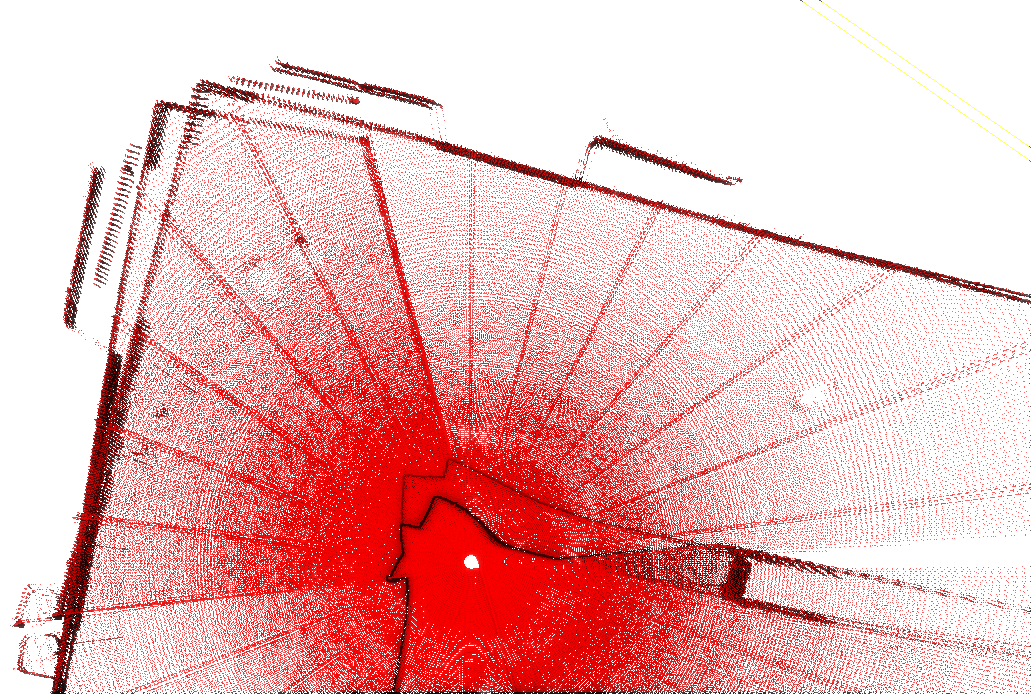
\includegraphics[width=0.7\textwidth]{uncallibrated-pointcloud}

    \caption{Uncalibrated point cloud of the capture 3.}
    \label{figure:uncallibrated-pointcloud}

\end{figure}

\subsubsection{RADLOCC}

The RADLOCC calibration, described in \cref{section:radlocc-method}, was the first method used to obtain the extrinsic calibration of the laser scanner. The evaluation of this calibration can be done by the re-projection of the laser scans onto the images, where the edges of the laser scan should be coincident with the edges of the chessboard, as seen in \cref{figure:radlocc-reprojection}. In total, six calibration datasets were obtained using the SICK LMS100 sensor, which have around 20 to 40 images and laser scans pairs. The results obtained are shown in table \cref{table:radlocc-results}.

\begin{figure}[h]
    
    \centering
    \begin{subfigure}{0.3\textwidth}
        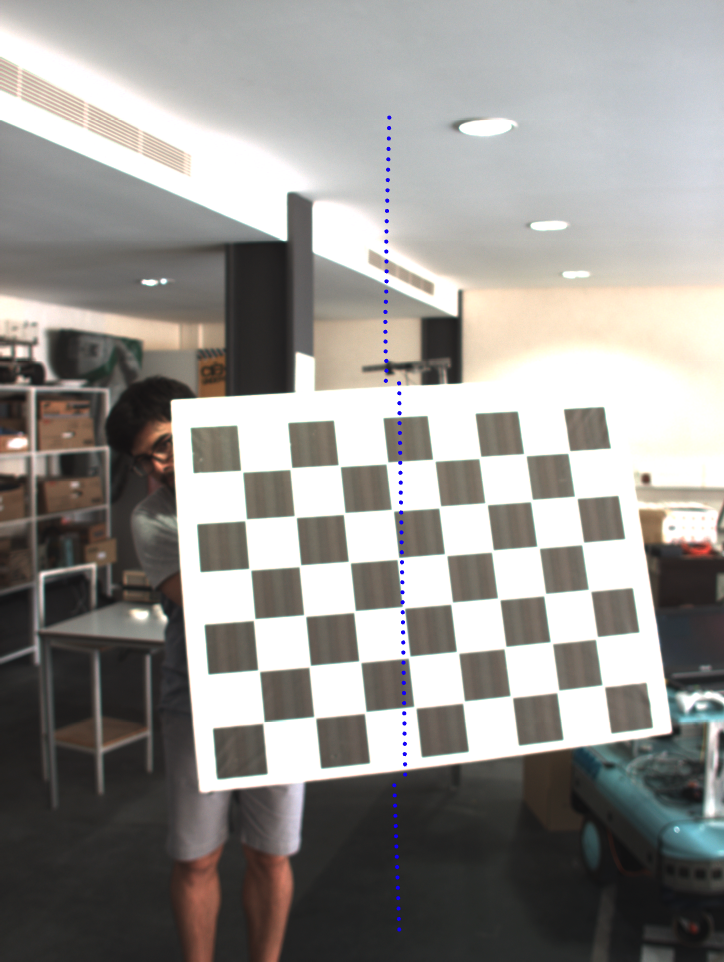
\includegraphics[height=6cm]{radlocc_calibration_1}
    \end{subfigure}%
    \begin{subfigure}{0.3\textwidth}
        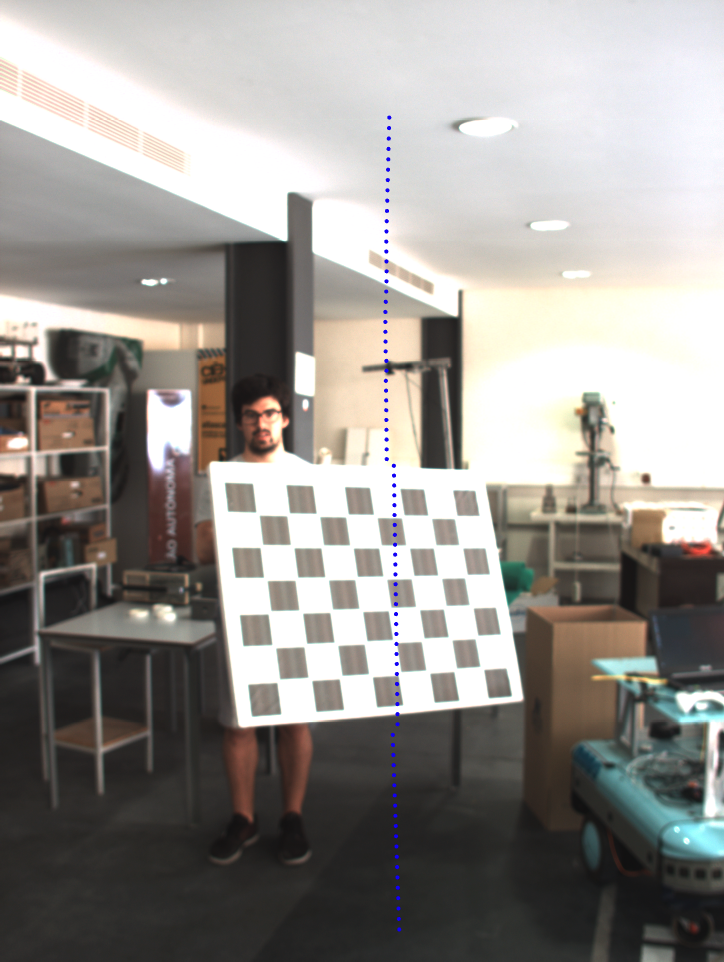
\includegraphics[height=6cm]{radlocc_calibration_2}
    \end{subfigure}%
    \begin{subfigure}{0.3\textwidth}
        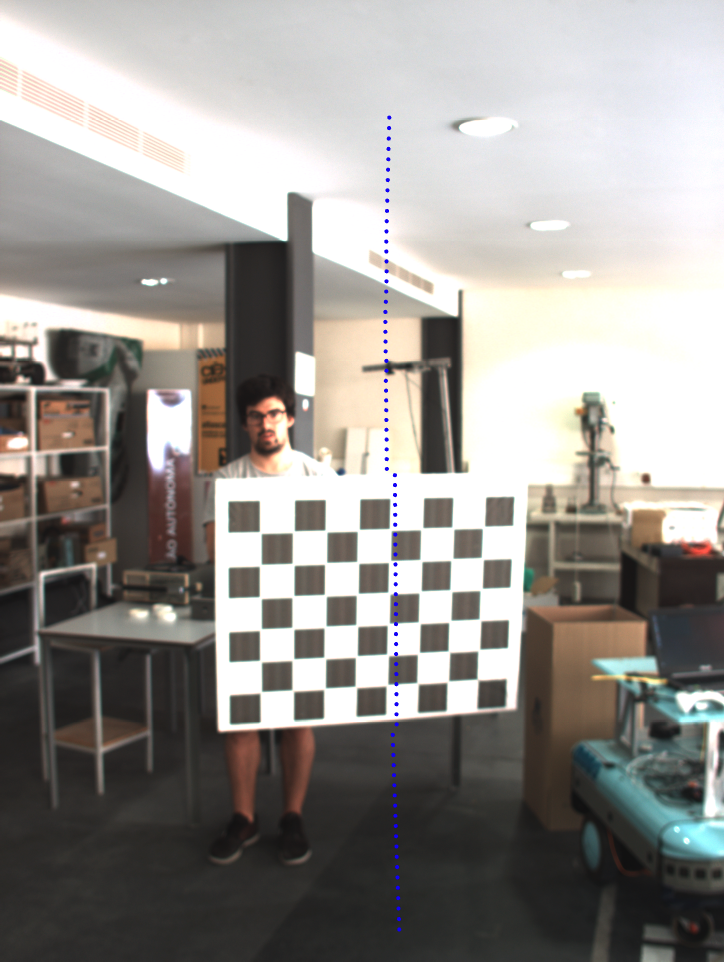
\includegraphics[height=6cm]{radlocc_calibration_3}
    \end{subfigure}%

    \caption{Reprojection of the laser scans in the images obtained in the RADLOCC calibration method.}

    \label{figure:radlocc-reprojection}

\end{figure}

\begin{table}[h]
    
    \caption{Resulting extrinsic calibration obtained using the RADLOCC method.}

    \centering
    \begin{tabu}{@{}c c ccc cccc@{}}
        \toprule
                &          & \multicolumn{3}{c}{translation} & \multicolumn{4}{c}{rotation} \\
                             \cmidrule(lr){3-5}\cmidrule(lr){6-9}
        Dataset & \#Images & $x$ & $y$ & $z$ & $x$ & $y$ & $z$ & $w$ \\
        \midrule
        1 & 28 & -0.0145 &  0.0435 & -0.0385 &  0.7129 & -0.0024 &  0.7008 & -0.0236 \\
        2 & 36 & -0.0242 &  0.0521 & -0.0926 &  0.7153 & -0.0082 &  0.6987 &  0.0059 \\
        3 & 38 &  0.0493 &  0.1823 & -0.0538 &  0.7113 &  0.0252 &  0.7005 &  0.0497 \\
        4 & 52 &  0.0190 &  0.0388 & -0.0561 &  0.7111 &  0.0005 &  0.7030 & -0.0077 \\
        5 & 15 & -0.0058 &  0.0850 & -0.0739 &  0.7183 &  0.0032 &  0.6956 & -0.0016 \\
        6 & 19 &  0.0072 & -0.0192 & -0.0334 &  0.7291 &  0.0247 &  0.6834 & -0.0245 \\
        7 & 14 &  0.0009 &  0.0699 & -0.0692 &  0.7126 &  0.0003 &  0.7013 & -0.0130 \\
        8 & 22 &  0.0212 &  0.0373 & -0.0641 &  0.7190 &  0.0074 &  0.6948 & -0.0131 \\
        \midrule
        $\mu^1$
            &  &  0.0066 &  0.0612 & -0.0602 &  0.7162 &  0.0063 &  0.6973 & -0.0034 \\
        $\sigma^2$
            &  &  0.0217 &  0.0539 &  0.0180 &  0.0056 &  0.0115 &  0.0059 &  0.0223 \\
        \bottomrule
        \multicolumn{5}{l}{$^1$ $\mu$ is the mean of the results.} \\
        \multicolumn{5}{l}{$^2$ $\sigma$ is the standard variation of the results.}

    \end{tabu}

    \label{table:radlocc-results}

\end{table}

It was expected to see similar results along the calibration, because the datasets were taken with similar conditions. However, there are large variations: for example, the translation on the $x$ axis between the dataset 2 and 3 has a difference of around \SI{0.07}{\meter}. This is not a negligible difference and, in the end, this can affect the geometry of the point cloud.

In conclusion, the resulting transformations have a large deviation between calibration, both in rotation and translation. This, associated with the fact that the full extrinsic calibration requires the extrinsic calibration of the camera, which also has significant error, justifies that this method is not suitable or capable for this application. 

\subsubsection{Planar Based Calibration Method}

The proposed method for the calibration uses the same data as the one used for the geometric reconstruction. The first step is the manual segmentation of the planes. At the end of this step, each point has a correspondent integer index, which is called the cluster index.  In figure \cref{figure:segmented-pointcloud-full}, a segmented point cloud can be seen, correspondent to the capture 3. Specifically, the deformation of this point cloud results can be as seen in \cref{figure:segmented-pointcloud-detail}.

\begin{figure}[h]
    
    \centering
    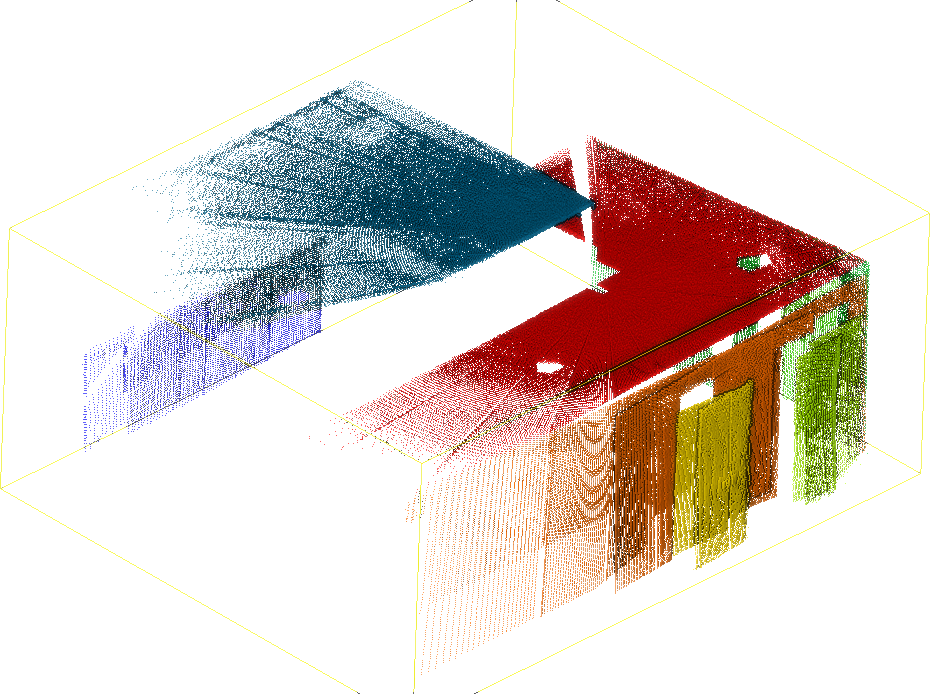
\includegraphics[width=0.8\textwidth]{segmented-pointcloud-full}
    \caption{Segmented point cloud from capture 3.}
    \label{figure:segmented-pointcloud-full}

\end{figure}

\begin{figure}[h]
    \centering
    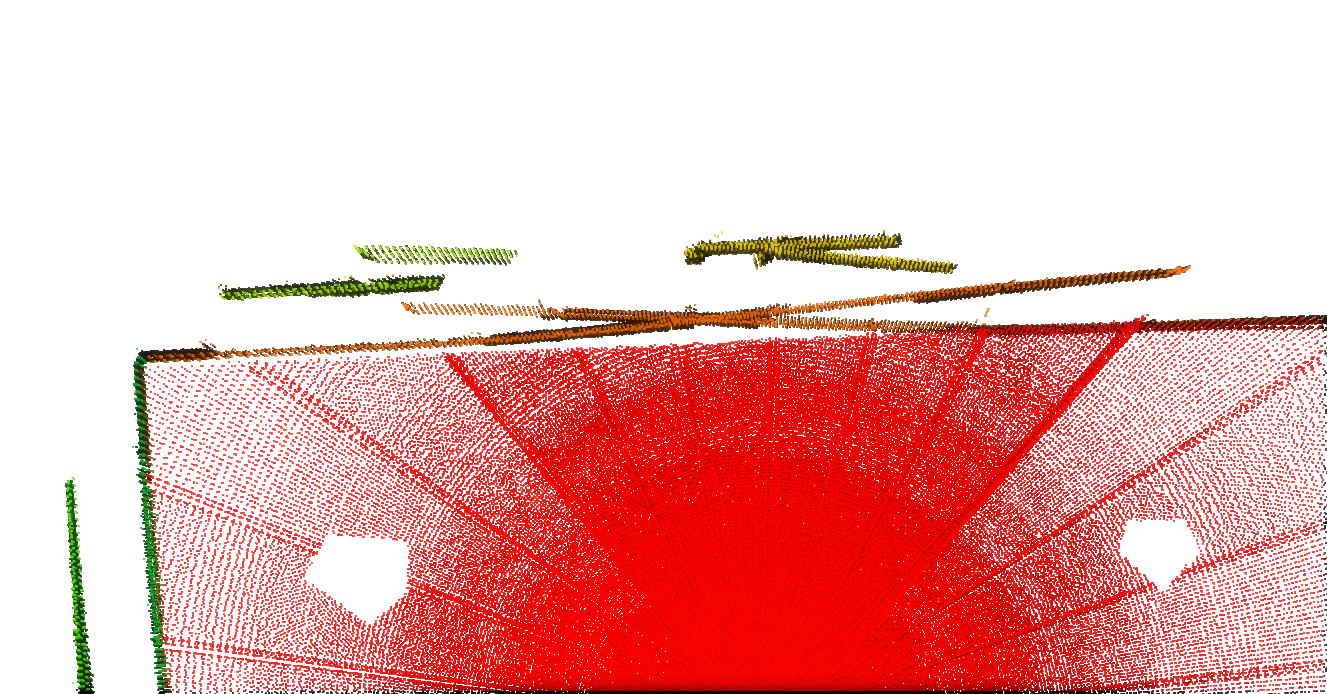
\includegraphics[width=0.8\textwidth]{segmented-pointcloud-detail}
    \caption{Detail of the segmented point cloud from capture 3.}
    \label{figure:segmented-pointcloud-detail}

\end{figure}

After the segmentation, the calibration score is minimized to obtain the extrinsic calibration of the laser scanner, as described in \cref{section:proposed-method}. For the initial estimate, a rough transformation was obtained via visual inspection. The result of a single acquisition is shown in \cref{figure:calibration-results-acquisition-3}. The initial score was \num{3.9e-3} and after 10 steps the score was reduced to about \num{1.1e-4}. The resulting point cloud at each step can be seen in \cref{figure:calibration-iterations}. The time required to this calibration is about \num{20}~minutes.

\begin{figure}[h]
    
    \centering
    \begin{subfigure}[t]{0.5\textwidth}
        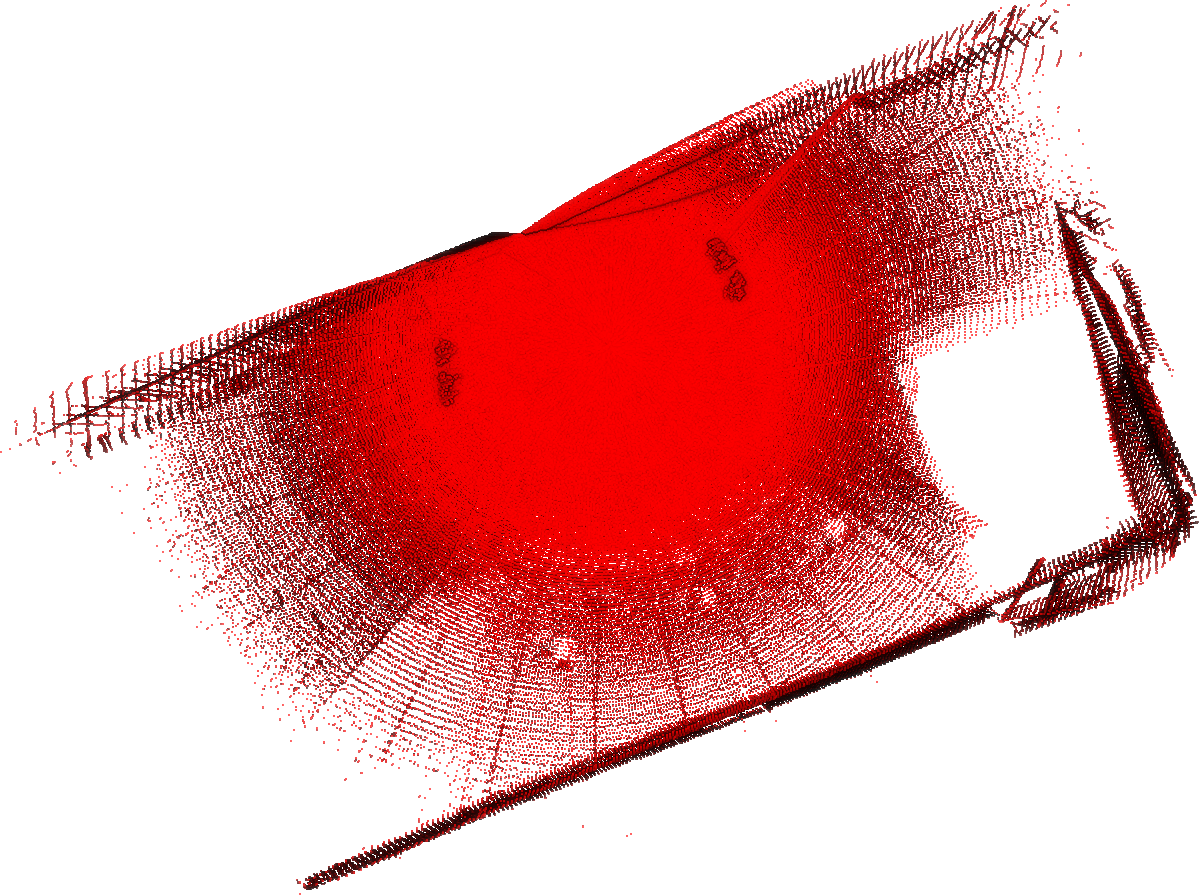
\includegraphics[width=\textwidth]{calibration-it-01}
        \caption{Iteration 1.}
        \label{figure:calibration-it-1}
    \end{subfigure}%
    \begin{subfigure}[t]{0.5\textwidth}
        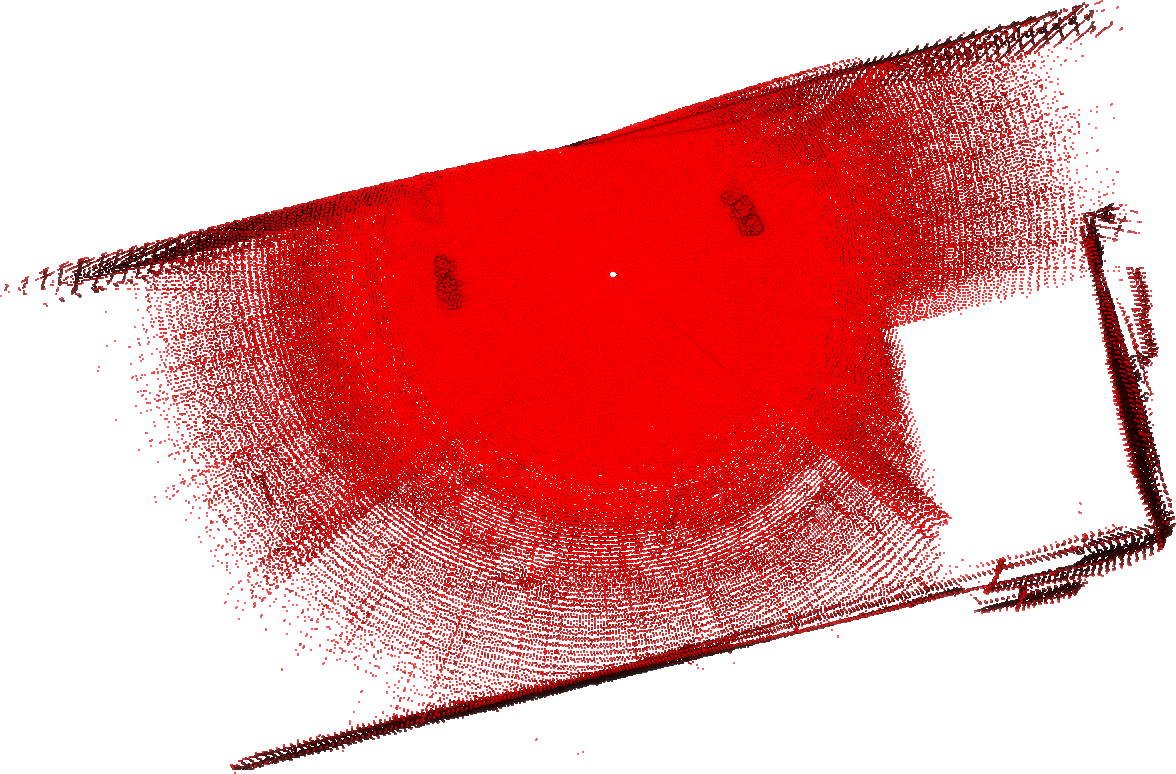
\includegraphics[width=\textwidth]{calibration-it-04}
        \caption{Iteration 4.}
        \label{figure:calibration-it-4}
    \end{subfigure}

    \begin{subfigure}[t]{0.5\textwidth}
        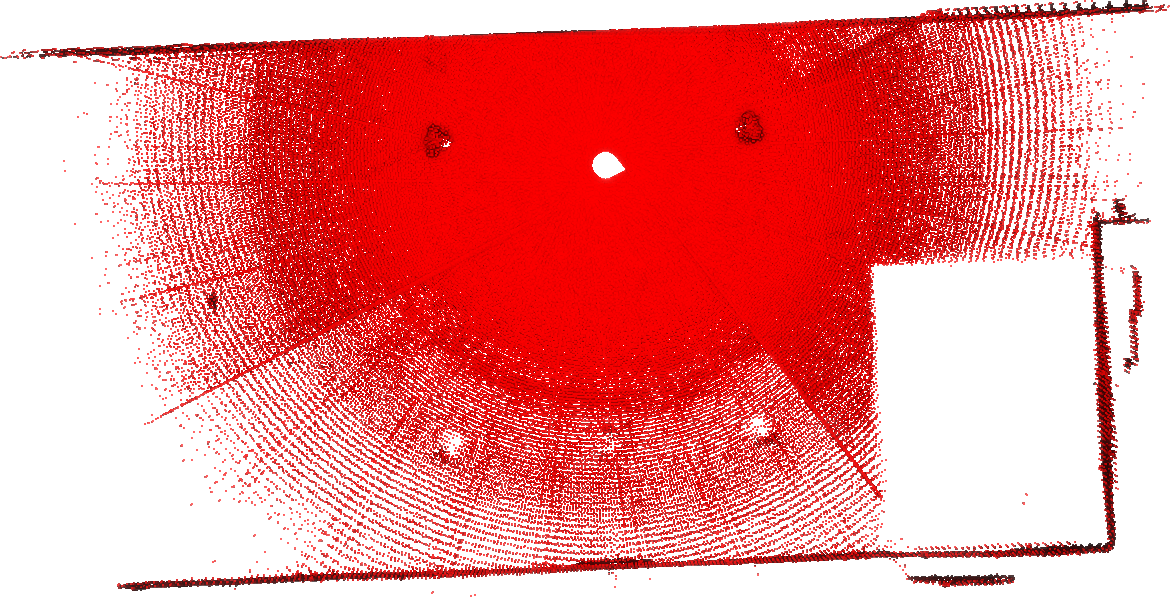
\includegraphics[width=\textwidth]{calibration-it-05}
        \caption{Iteration 5.}
        \label{figure:calibration-it-5}
    \end{subfigure}%
    \begin{subfigure}[t]{0.5\textwidth}
        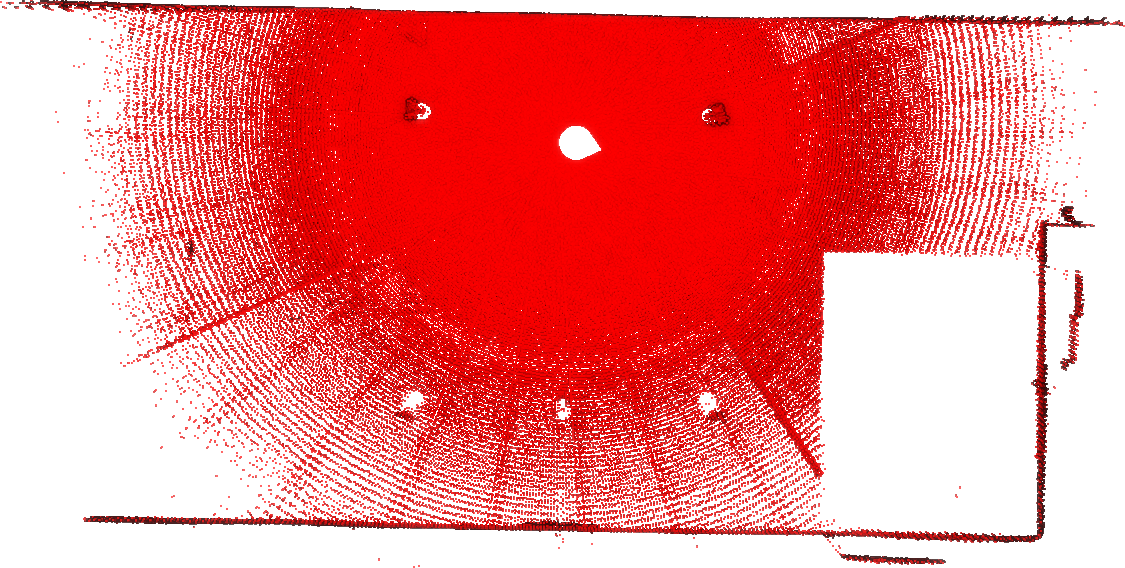
\includegraphics[width=\textwidth]{calibration-it-07}
        \caption{Iteration 7.}
        \label{figure:calibration-it-7}
    \end{subfigure}

    \caption{Resulting point cloud at each iteration in the optimization process.}
    \label{figure:calibration-iterations}

\end{figure}

\begin{figure}[h]

    \centering
    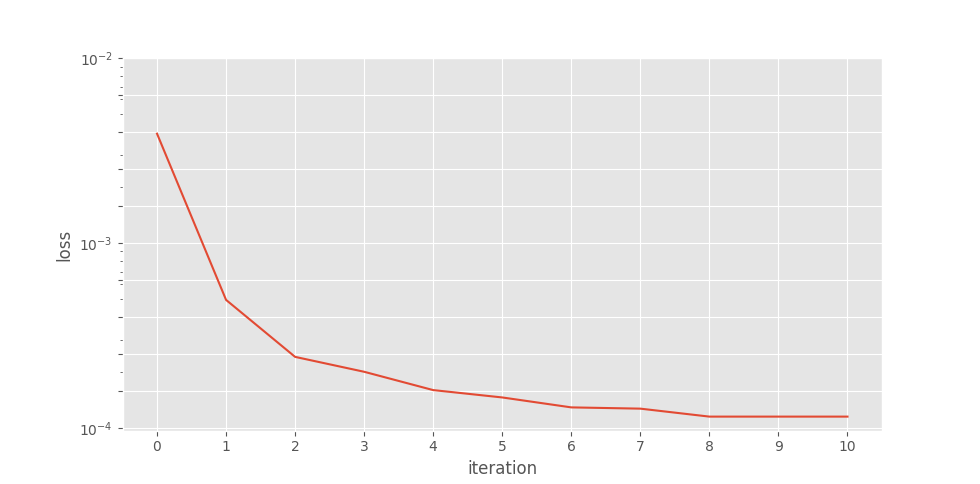
\includegraphics[width=0.7\textwidth]{calibration-iterations}
    
    \caption{Calibration iteration results for the third acquisition of the capture 4.}
    \label{figure:calibration-results-acquisition-3}
\end{figure}

The resulting calibration does indeed improve the geometry of the point cloud, shown before. In \cref{figure:calibration-comparison}, the resulting point cloud (in red) can be compared to the previous point cloud, obtained by the initial estimate. As can be seen, the deformation visible before are no longer present in the calibrated point cloud.

\begin{figure}[h]
    \centering
    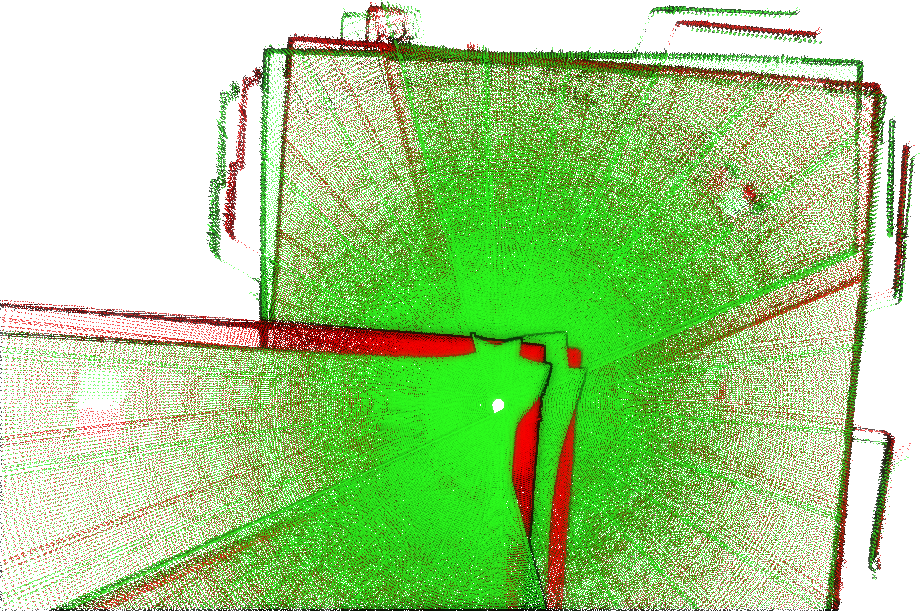
\includegraphics[width=\textwidth]{calibration-comparison}
    \caption{Comparison between the calibrated point cloud (in red) and the non-calibrated point cloud (in green).}
    \label{figure:calibration-comparison}
\end{figure}

In general, this calibration method successfully yields similar results for different acquisitions and captures. In other words, the calibration is repeatable. For example, the transformations obtained for a set of acquisitions of the capture 5 has similar results across the acquisitions, as shown in \cref{table:extrinsic-calibration-multiple-acquisitions}.

As seen, the standard deviation $\sigma$ in this calibration is much less that in the RADLOCC calibration. For example, in the translation in the $x$ axis, in RADLOCC $\sigma \approx \SI{0.02}{\meter}$, while in this calibration it was $\sigma \approx \SI{0.002}{\meter}$, which is approximately ten times less.

\begin{table}
    \caption{Extrinsic calibration obtained using multiple acquisitions.}

    \centering
    \begin{tabu}{@{}c ccc c cccc@{}}
        \toprule
                    & \multicolumn{3}{c}{translation} & &  \multicolumn{4}{c}{rotation} \\
                             \cmidrule(lr){2-4}\cmidrule(lr){5-9}
        Acquisition & $x$ & $y$ & $z$ & & $q_x$ & $q_y$ & $q_z$ & $q_w$ \\
        \midrule
            1 & -0.00157 & 0.1195 & 0.1053 & & -0.5015 & -0.5151 & -0.5056 & 0.4770 \\
            2 &  0.00401 & 0.1103 & 0.0932 & & -0.5006 & -0.5175 & -0.5035 & 0.4776 \\
            3 &  0.00301 & 0.1222 & 0.0982 & & -0.5001 & -0.5168 & -0.5042 & 0.4782 \\
            4 &  0.00434 & 0.1321 & 0.0988 & & -0.5014 & -0.5158 & -0.5059 & 0.4761 \\
        \midrule
        $\mu$    & 0.00245 & 0.12103 & 0.09888 & & -0.50090 & -0.51630 & -0.50480 & 0.47723 \\
        $\sigma$ & 0.00237 & 0.00777 & 0.0043  & & 0.00058 & 0.00092 & 0.00099 & 0.00078 \\
        \bottomrule

    \end{tabu}

    \label{table:extrinsic-calibration-multiple-acquisitions}
\end{table}

Therefore, the proposed calibration can be a reliable method to obtain the extrinsic calibration of laser scanners mounted in motion platforms, as the PTU, because transformation obtained has the accuracy required for the geometric registration of the laser scanners for this work and the results have repeatability and reproductivity. The advantages of this method, compared to the previous method, are:

\begin{enumerate}
    \item The method directly obtains the extrinsic transformation of the laser scanner, instead of a partial transformation (to the camera). This also decreases the error that would come from the intrinsic and extrinsic calibration of the camera.
    \item This calibration uses exclusively the laser scanner data, which is more accurate than images, because it is a direct measurement, as opposed to the transformation resulting from a pose estimation algorithm. Moreover, the number of laser scans used are also greater than in the RADLOCC method, which can explain the smaller error found in this calibration method.
    \item This calibration acknowledges and benefits from the movement of the PTU, as opposed to the RADLOCC, which was designed for static laser scanners. The laser scanner has to be static in RADLOCC, so that the background segmentation of the laser scans is possible.
    \item The method proposed uses the data from the acquisitions directly, so the calibration process can be done even after the capture is made, or if the laser scanner is not available. This can be useful if the prior calibration did not have the accuracy required for the acquisition, for example, if the calibration was done using a smaller scene, or if the equipment has changed or is not available. The only requirement is that there are enough planes in the scene for the calibration.
\end{enumerate}

\subsection{Normal Estimation}
\label{section:results-normal-estimation}

In this section, the results obtained from the Normal Estimation method described in \cref{section:normal-estimation} are shown and compared to the more traditional method using the $k$-nearest-Neighbors. Both methods have similar results, as shown in \cref{figure:normal-estimation-results}, however, there are differences:

\begin{enumerate}
    \item The proposed method relies on a continuous movement in pan, while recording the laser scans. However, this was not the case for the acquisitions, because the movement was interrupted to record the images. This can explain why some points have the wrong normals. However, this limitation can be surpassed if the movement of the PTU is continuous.
    \item This method can only be used for each acquisition and can not be generalized for any point cloud, because it required that the point cloud is structured in a 2D structure. The other method, however, works for any point cloud.
    \item The computational complexity of the proposed method is $O(N)$, while the complexity of the method using the $k$-Neighbors is $O(N \log N)$, which has an increasing impact for large point clouds. For example, in a point cloud with 5 million points (for example, in captures 5 and 6), the time required to calculate the normals using the proposed method is \SI{10}{\second} (using a implementation in python, which is regarded as a slow language for numerical computations) and using the $k$-neighbors method the time required is about \SI{10}{\minute}.
\end{enumerate}

\begin{figure}[h]
    
    \centering
    \begin{subfigure}[t]{\textwidth}
        \centering
        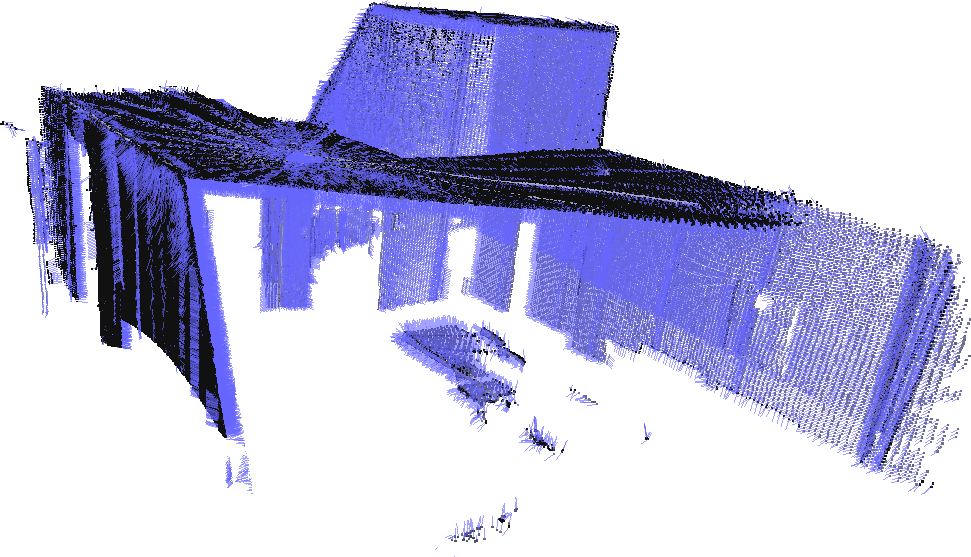
\includegraphics[width=0.7\textwidth]{normals-estimation-method}
        \caption{Normal estimation result using the proposed method.}
        \label{figure:normals-estimation-method}
    \end{subfigure}

    \begin{subfigure}[t]{\textwidth}
        \centering
        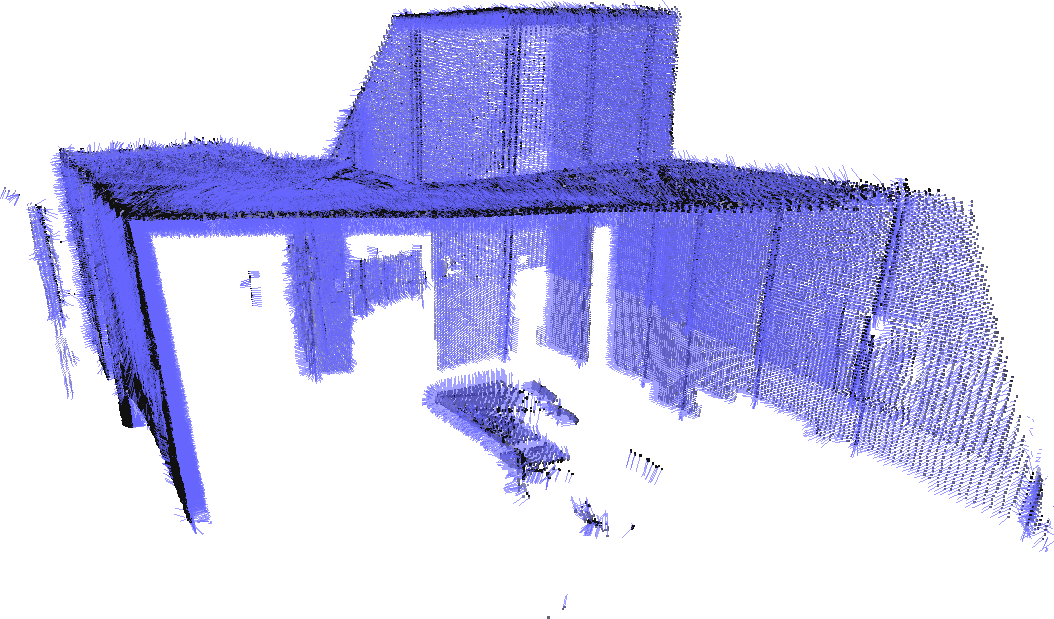
\includegraphics[width=0.7\textwidth]{normals-estimation-other-method}
        \caption{Normal estimation result using the common method.}
        \label{figure:normals-estimation-other-method}
    \end{subfigure}

    \caption{Comparison of both Normal estimation methods (the blue arrows represent the normal vector).}
    \label{figure:normal-estimation-results}

\end{figure}

\subsection{Acquisition Registration}

The method for the acquisition registration uses the ICP algorithm, which find the transformation between two point clouds by the minimization of the distance between the point clouds. However, finding the closest points in the two point clouds is a difficult task and can be wrong if two point clouds are far apart. In particular, the point clouds transformation is the distance between the acquisition poses, which is in the order of meters. The ICP method, however, is only successful if the manual alignment is already very close. Any noticeable misalignment results in a wrong registration, as seen in \cref{figure:icp-results}. The solution found was to manually align the point clouds first, and then use the ICP algorithm as a fine alignment. This solution is sub-optimal, as it is not automatic, thus requiring manual work. These shortcomings in the acquisition registration can be solved by either enhancing the ICP algorithm to improve the registration for large differences, or by providing the inicial estimate for the transformation between each acquisition.

\begin{figure}[h]
    
    \centering
    \begin{subfigure}[t]{0.5\textwidth}
        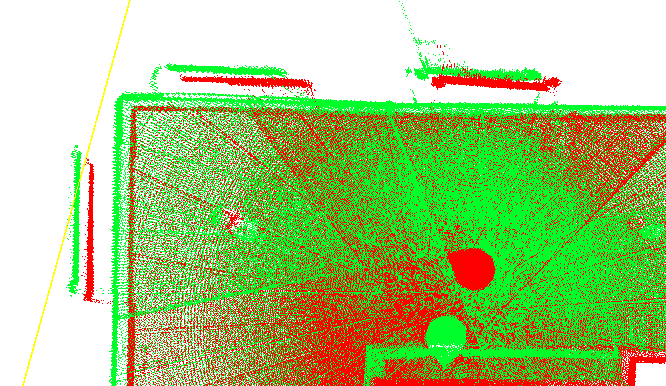
\includegraphics[width=\textwidth]{icp-registration-wrong-before}
        \caption{Before the ICP registration (incorrect).}
        \label{figure:icp-registration-wrong-before}
    \end{subfigure}%
    \begin{subfigure}[t]{0.5\textwidth}
        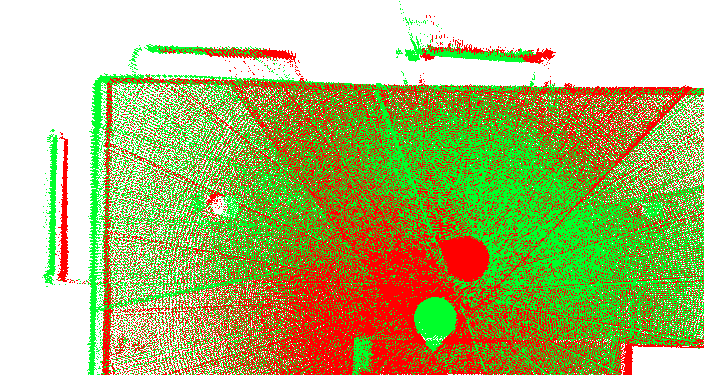
\includegraphics[width=\textwidth]{icp-registration-wrong-after}
        \caption{After the ICP registration (incorrect).}
        \label{figure:icp-registration-wrong-after}
    \end{subfigure}

    \begin{subfigure}[t]{0.5\textwidth}
        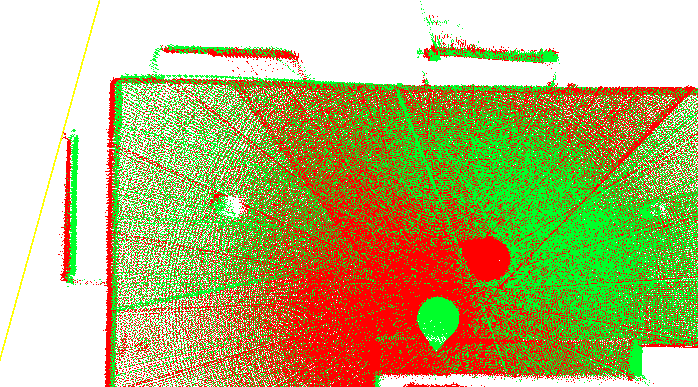
\includegraphics[width=\textwidth]{icp-registration-right-before}
        \caption{Before the ICP registration (correct).}
        \label{figure:icp-registration-right-before}
    \end{subfigure}%
    \begin{subfigure}[t]{0.5\textwidth}
        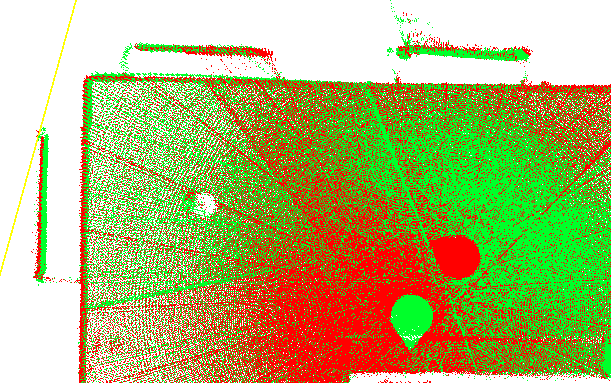
\includegraphics[width=\textwidth]{icp-registration-right-after}
        \caption{After the ICP registration (correct).}
        \label{figure:icp-registration-right-after}
    \end{subfigure}

    \caption{Comparison of the results regarding the ICP registration for different initial estimates. Two registration with a small difference result (\cref{figure:icp-registration-right-before,figure:icp-registration-wrong-before}) can yield two different outcomes (\cref{figure:icp-registration-right-after,figure:icp-registration-wrong-after}).}
    \label{figure:icp-results}

\end{figure}

Another disadvantage of the ICP algorithm is that the registration is pairwise. In this work, multiple point clouds were registered, and the inability of the ICP to register more than two point clouds at once implies that the registration does not use the full spectrum of data available, and is constrained to only the two point clouds at each registration. This suggests that a registration which is done between two point clouds with small overlap, which results in a weaker registration, could be avoided. If the algorithm used the entire data set, the registration would be done with the most overlap possible, and number of common points is maximized. To circumvent this problem, the three alternative methods are shown in \cref{section:acquisition-registration}. 

However, only the second method was proven to be effective in this work. This method registers the point clouds to an accumulated point cloud resulted by the fusion of the prior registered point clouds. The success of this method can be explained by the increasing overlap existent in further registrations. The other methods fail because there are point clouds that have so small overlap that the ICP method always fail. For example, in the \cref{figure:icp-methods}, two registrations are done, where the target point cloud is colorized in red. As seen, the registration fails in the pairwise registration (against other point cloud in green), but is successful when the reference point cloud is the accumulated point cloud (in green).

\begin{figure}[h]
    
    \centering
    \begin{subfigure}[t]{0.5\textwidth}
        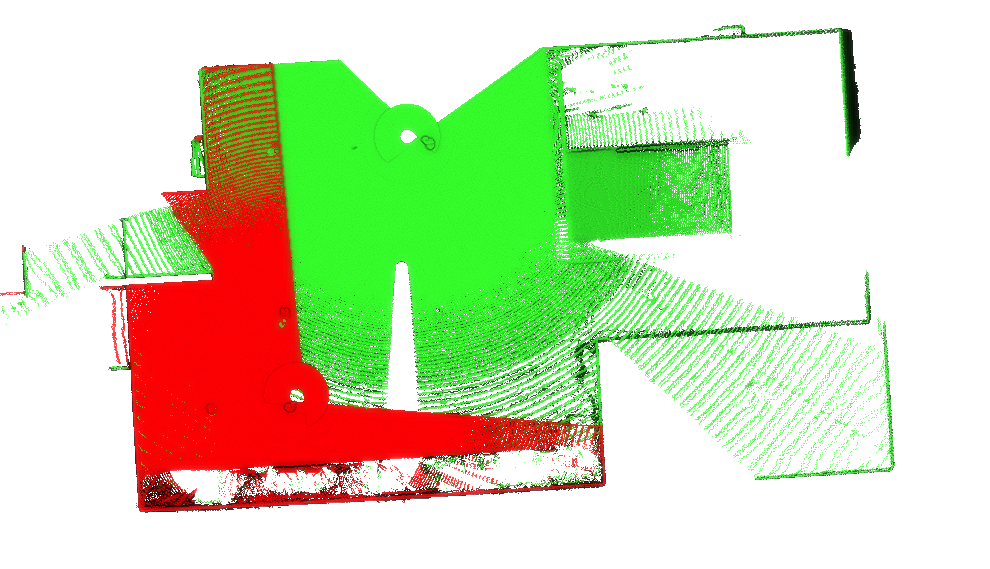
\includegraphics[width=\textwidth]{icp-error-before}
        \caption{Pairwise registration (before).}
        \label{figure:icp-method-1-wrong}
    \end{subfigure}%
    \begin{subfigure}[t]{0.5\textwidth}
        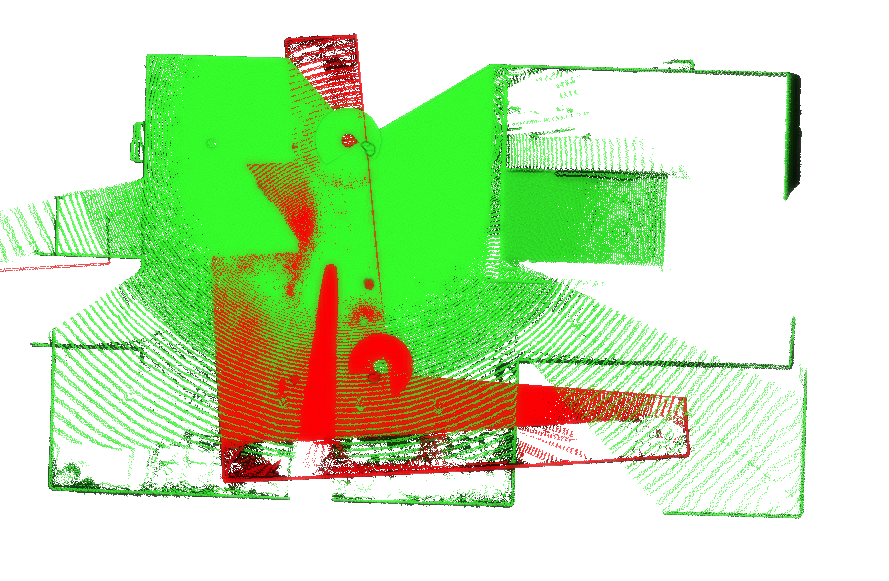
\includegraphics[width=\textwidth]{icp-error-after}
        \caption{Pairwise registration (after).}
        \label{figure:icp-method-1-right}
    \end{subfigure}

    \begin{subfigure}[t]{0.5\textwidth}
        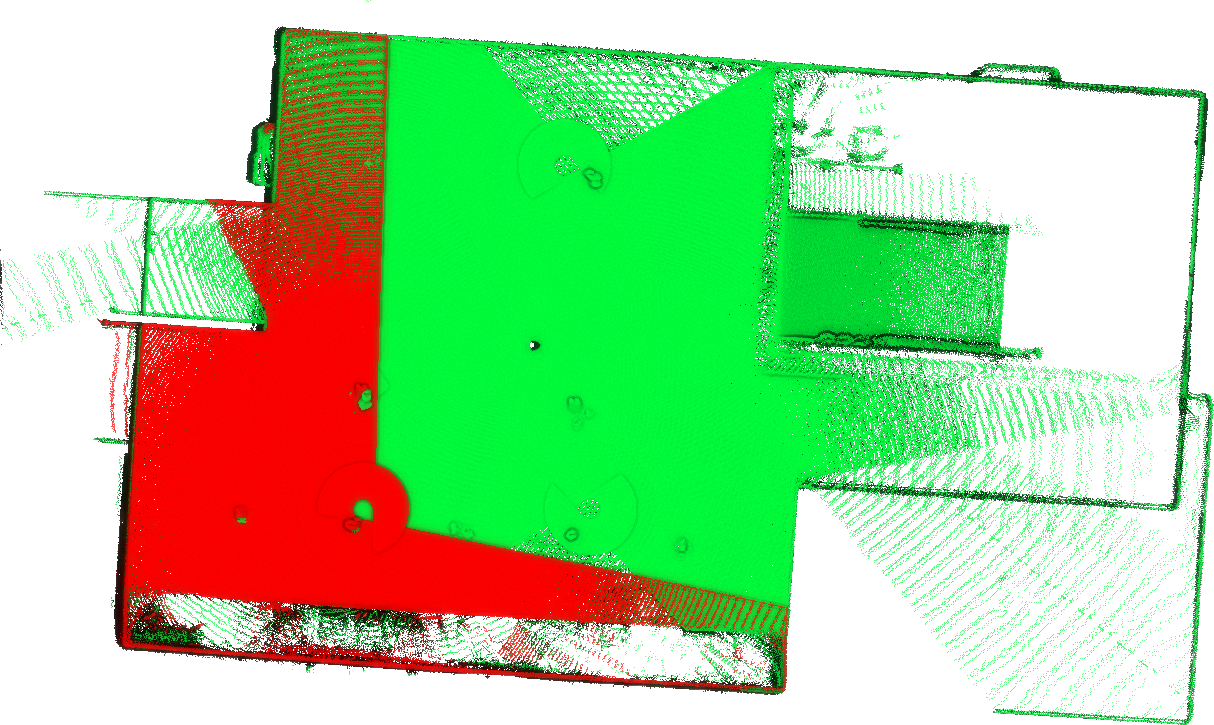
\includegraphics[width=\textwidth]{icp-accumulated-before}
        \caption{Accumulated registration (before).}
        \label{figure:icp-method-2-before}
    \end{subfigure}%
    \begin{subfigure}[t]{0.5\textwidth}
        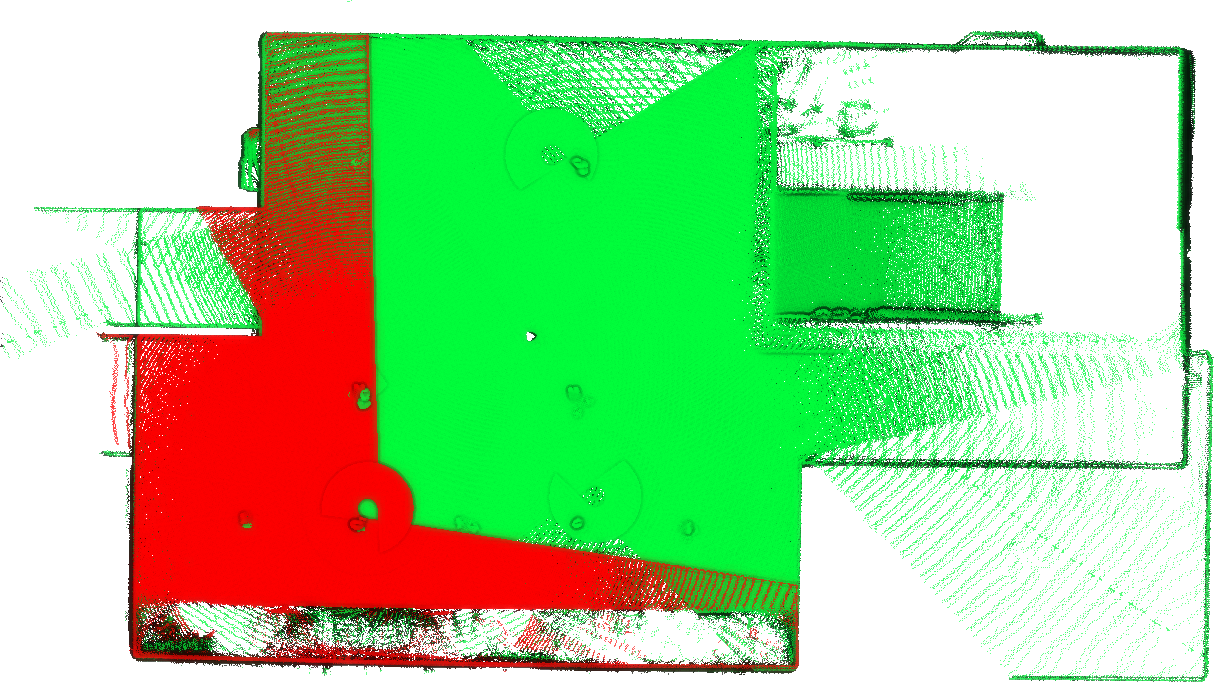
\includegraphics[width=\textwidth]{icp-accumulated-after}
        \caption{Accumulated registration (after).}
        \label{figure:icp-method-2-after}
    \end{subfigure}

    \caption{Comparison of the ICP registration between two point clouds or between the accumulated point cloud and another point cloud.}
    \label{figure:icp-methods}

\end{figure}

In conclusion, the ICP algorithm is not sufficient for an automatic registration of the acquisitions. However, with manual intervention as a first registration, the ICP algorithm can be used to find the fine registration of the acquisitions. Using this method, the registrations were possible, as shown in \cref{figure:icp-results}.

\begin{figure}[h]
    
    \centering
    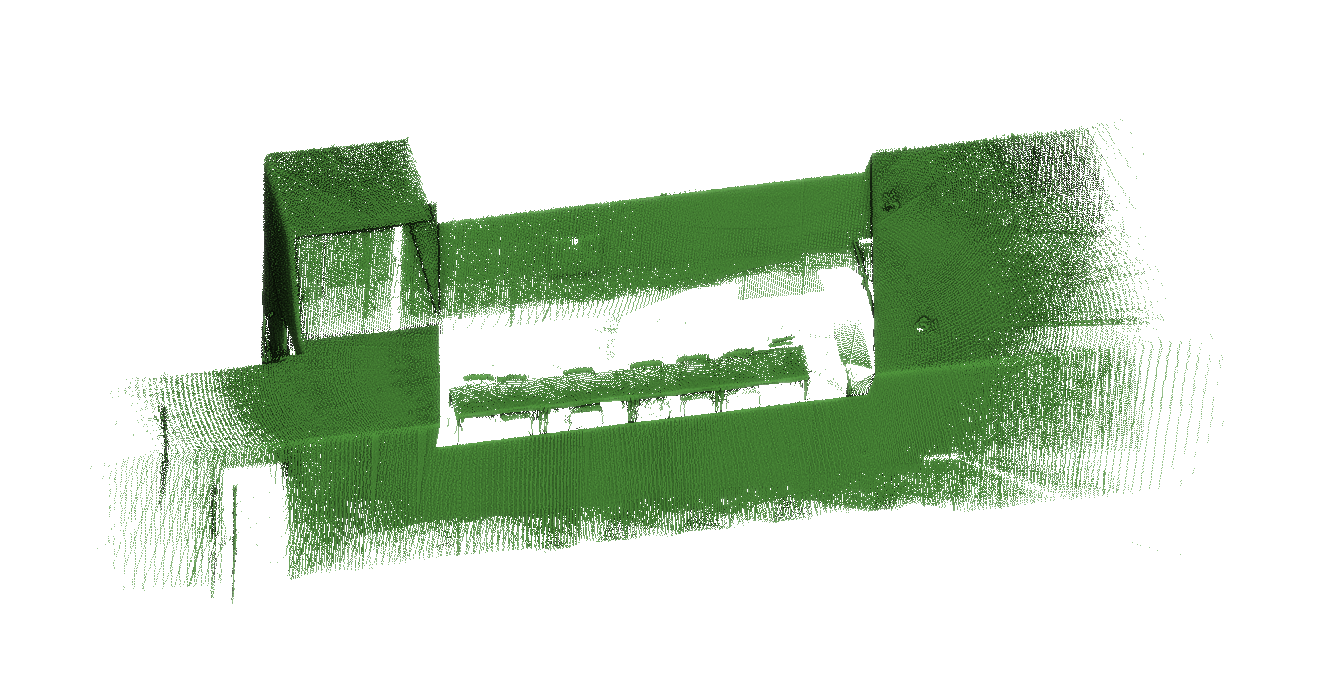
\includegraphics[width=\textwidth]{icp-result}

    \caption{Resulting fusion of all point clouds obtained in the capture 3, after the acquisition registration.}
    \label{section:icp-result}

\end{figure}

\subsection{Influence of the different laser scanners}

In this work, three different laser scanners were used to study the influence of the different characteristics of each one on the reconstruction process.

The aperture of the laser and the range are important factors in the capture process. As an example, the Hokuyo URG04 has a small range of \SI{5.6}{\meter}, compared to the larger range of the two other lasers, which both have a range of \SI{30}{\meter}. The resulting point clouds are, then, much smaller in the case of the Hokuyo~URG04, which means that more acquisitions are required to capture a scene, and the distance between each acquisition should not be larger that the range of the laser scanner. Otherwise, there is no overlap between acquisitions so the acquisition registration would fail. The same can be applied to the aperture of the laser scanner. 

Also, the response of the same surfaces differ from laser to laser, mostly due to the wavelength and energy of the laser used. As an example, the floor surface, which was made of tiles with reflective material, was only properly registered in the SICK LMS100 laser scanner, which is the laser with the most power output. It is expected to be due to the high reflection of the surface, only a small fraction of the laser beams is reflected back to the laser scanner. If the laser emitted does not have considerable power, the reflected light could not have sufficient energy to be detected by the sensor. 

Moreover, the scanning rate of the laser scanner can be important to obtain dense point clouds, without requiring a large acquisition time. The Hokuyo UTM30 was the laser scanner with the higher scanning rate (\SI{40}{\hertz}), which produced point clouds with about 4 times the number of points obtained by the two other lasers, without sacrificing the acquisition time.

Lastly, a problem was identified in the SICK LMS100 laser which made it unsuitable for this application, because the laser scans obtained were not accurate, compared to the other sensors. The laser scans of planar surfaces appear as deformed in this laser scanner. This can be seen in \cref{figure:deformed-laser}, where both the floor and the root are not shown as curved lines. Therefore, the resulting point clouds were always deformed, even after many extrinsic calibrations. This is most probably a problem of this laser scanner, and it is suspected to be due to a damaged laser scanner. Therefore, the acquisitions of this laser are not considered further on.

\begin{figure}[h]
    
    \centering
    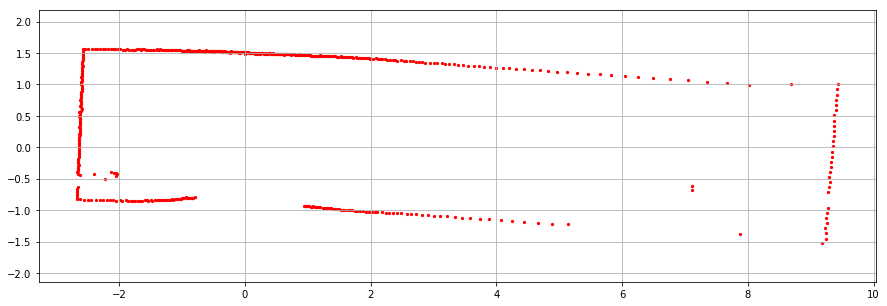
\includegraphics[width=\textwidth]{laser-deformation}

    \caption{Deformed laser of the LMS100 laser scanner.}
    \label{figure:deformed-laser}

\end{figure}

\subsection{Overall Results}

The results of the geometric registration are satisfactory, mostly because of the new calibration method of the laser, which ensured the success all the geometric algorithms used further on, such as the normal estimation and the acquisition registration. The overall results are shown in \cref{figure:results-capture-5,figure:results-capture-6}.


\begin{figure}[h]

    \centering
    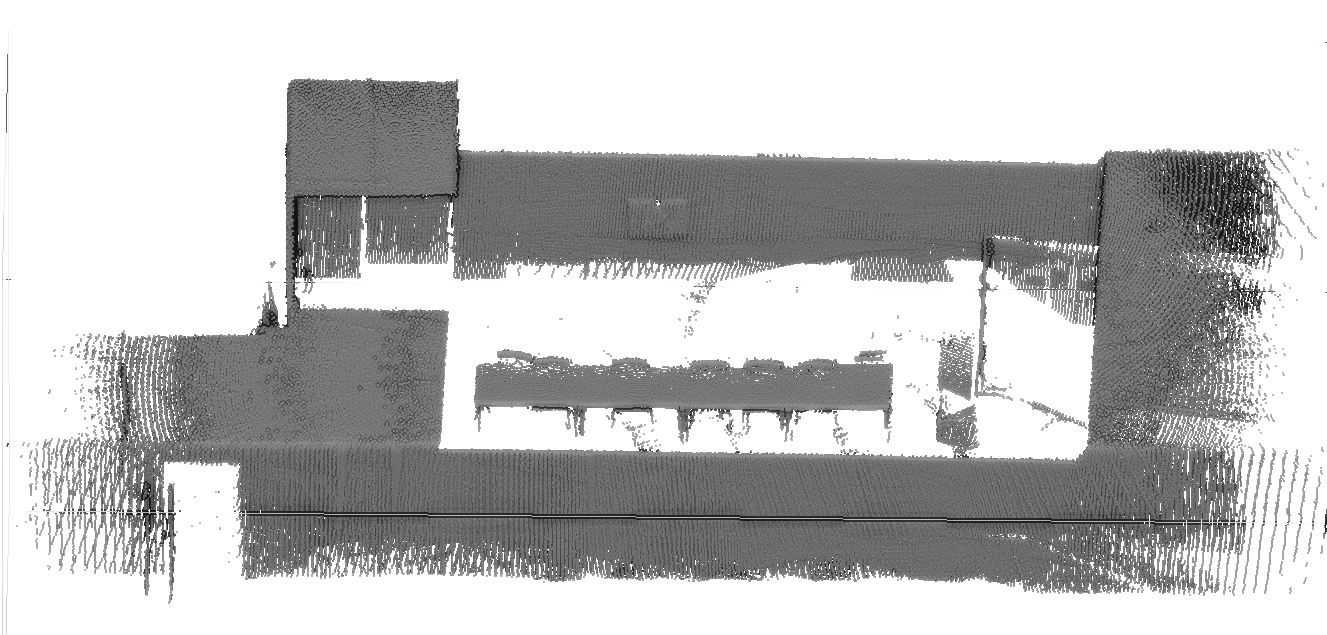
\includegraphics[width=\textwidth]{geometry-result-2}

    \caption{Result of the geometric reconstruction of the capture 5.}
    \label{figure:results-capture-5}
    
\end{figure}

\begin{figure}[h]

    \centering
    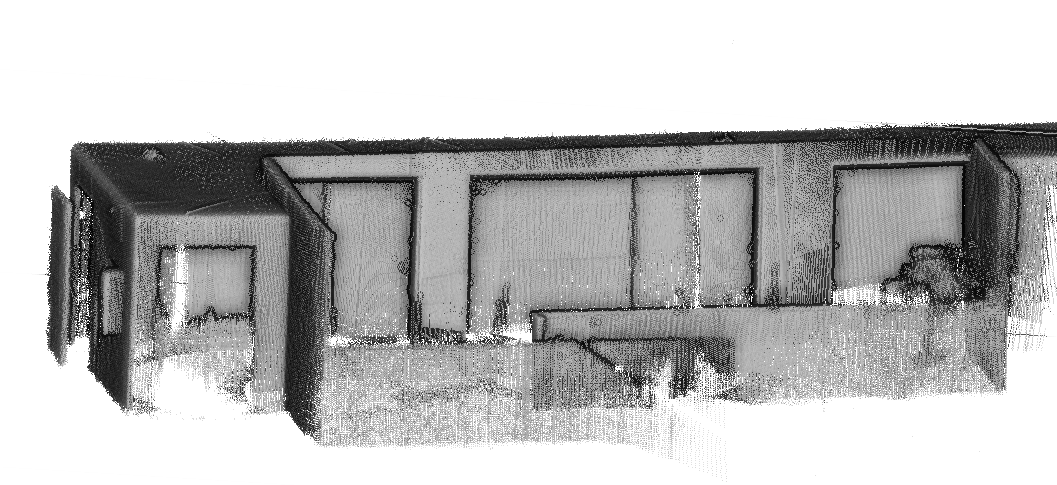
\includegraphics[width=\textwidth]{geometry-result-1}

    \caption{Result of the geometric reconstruction of the capture 6.}
    \label{figure:results-capture-6}
    
\end{figure}

\section{Color Reconstruction}

The color reconstruction is the final part of the reconstruction, which uses the images taken from the camera and registers the color into the point cloud obtained in the geometric reconstruction and merges the colors to obtain a colorized point cloud. This methods require both the intrinsic and extrinsic calibration of the camera, to register the images correctly. 

\subsection{Camera Intrinsic Calibration}

This calibration obtains the intrinsic parameters of the camera, as the focal length and center point. This calibration method used is widely used so it is expected that the results are accurate. 

\subsection{Camera Extrinsic Calibration}

The method used to obtain the extrinsic calibration of the camera was the hand-in-eye calibration method. In this work, an ArUCO marker with a side of \SI{200}{\milli\meter} was placed about \SI{2}{\meter} away from the camera. The PTU was then manually controlled to capture different images of the marker in different poses of the camera. After about 30 poses, the calibration was done. The number of calibration done using this method were 3, and the results are shown in \cref{table:camera-extrinsic-calibration-results}. The results are very close between calibrations: for example, the standard deviation in the translation is in the order of \SI{0.001}{\meter}.

\begin{table}[h]
    \caption{Results of the extrinsic calibration of the camera.}

    \centering
    \begin{tabu}{@{}l ccc cccc @{}}
        \toprule
            &       \multicolumn{3}{c}{translation} & \multicolumn{4}{c}{rotation} \\
                             \cmidrule(lr){2-4}\cmidrule(lr){5-8}
        calibration &  $x$ &  $y$ &  $z$ &  $q_x$ &  $q_y$ &  $q_z$ & $q_w$ \\
        \midrule
        0 & -0.103524 &      -0.086451 &       0.050509 & 0.027264 &   -0.702682 &   -0.024205 &  0.710570 \\
        1 & -0.100458 &      -0.088829 &       0.049478 & 0.030372 &   -0.701046 &   -0.027414 &  0.711941 \\
        2 & -0.098975 &      -0.084319 &       0.046249 & 0.033105 &   -0.702234 &   -0.031446 &  0.710481 \\
        3 & -0.101184 &      -0.089208 &       0.052215 & 0.029564 &   -0.702891 &   -0.025002 &  0.710243 \\
        \midrule
        $\mu$
          & -0.10104  &      -0.087202 &       0.049613 & 0.030076 &   -0.702213 &   -0.027017 &  0.710808 \\
        $\sigma$
          & 0.001643  &       0.001971 &       0.002174 & 0.002088 &    0.000714 &    0.002817 &  0.000665 \\
        \bottomrule
        \end{tabu}


    \label{table:camera-extrinsic-calibration-results}
\end{table}

However, this calibration lacks the required precision for the color registration, because the colors are noticeable misaligned with the geometry, as seen in the next section. The failure of this calibration can be related to multiple shortcomings in this calibration method. First, this calibration uses an ArUCO as the marker for the pose estimation. It is possible that the error associated with the pose estimation is large and be the source of the error of the calibration. Second, the limited field of view of the camera limits the range of the movements of the PTU for a small interval of angles in pan and tilt. This limitation in space can result in a limited space of angles registered, which can therefore impact the accuracy of the result. It is possible that, by using more markers, wider angles cloud be possible. Hence, this calibration fails to obtain an accurate extrinsic calibration of the camera.

\FloatBarrier

\subsection{Color Registration and Fusion}

In the color registration and fusion process, the color is attributed to each point in the point cloud. In short, the color registration defines how each point is colorized, based on an image, and the fusion process defines what is the resulting color, after all the images are registered. In total, six methods were tested in this work for the color fusion: the first three methods choose a color from all the registered color and the last two methods calculate the average of all the colors, though a simple mean, or a weighted mean.

The registration process was, however, not perfect, mostly due to a imperfect calibration of the camera. Therefore, the color are not registered in their correct positions, as seen in \cref{figure:wrong-registration-photocopy}. In this image, the colors from different object are registered in wrong objects, for example, the elevator door. This is a common problem and can be seen, for example, in the elevator door.

\begin{figure}[h]
    
    \centering
    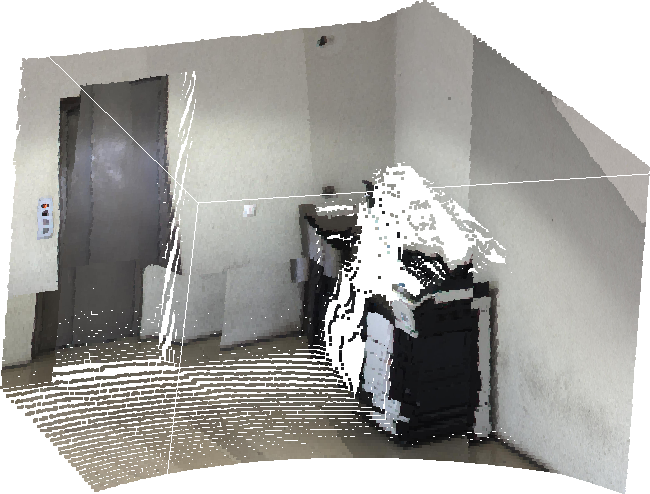
\includegraphics[width=0.6\textwidth]{color-registration-1}

    \caption{Example of the inaccurate color registration.}
    \label{figure:wrong-registration-photocopy}
\end{figure}

Also, the images taken have different color values for the same objects. This is due to illumination differences at the capture of each image. This difference is also noticed in the colorized point clouds. This problem is hard to solve, but can be mitigated by ensuring an uniformly illuminated scene. Even so, direct sunlight or shadows negatively affect the colorization. This problem can be shown is the images in \cref{figure:illumination-issues-images}, where the differences in color are very noticeable. The resulting colorization has, therefore, the same variation in color as the one present in the images, as shown in \cref{figure:illumination-issues-pointcloud}.

\begin{figure}[h]
    
    \centering
    \begin{subfigure}{0.5\textwidth}
        \centering
        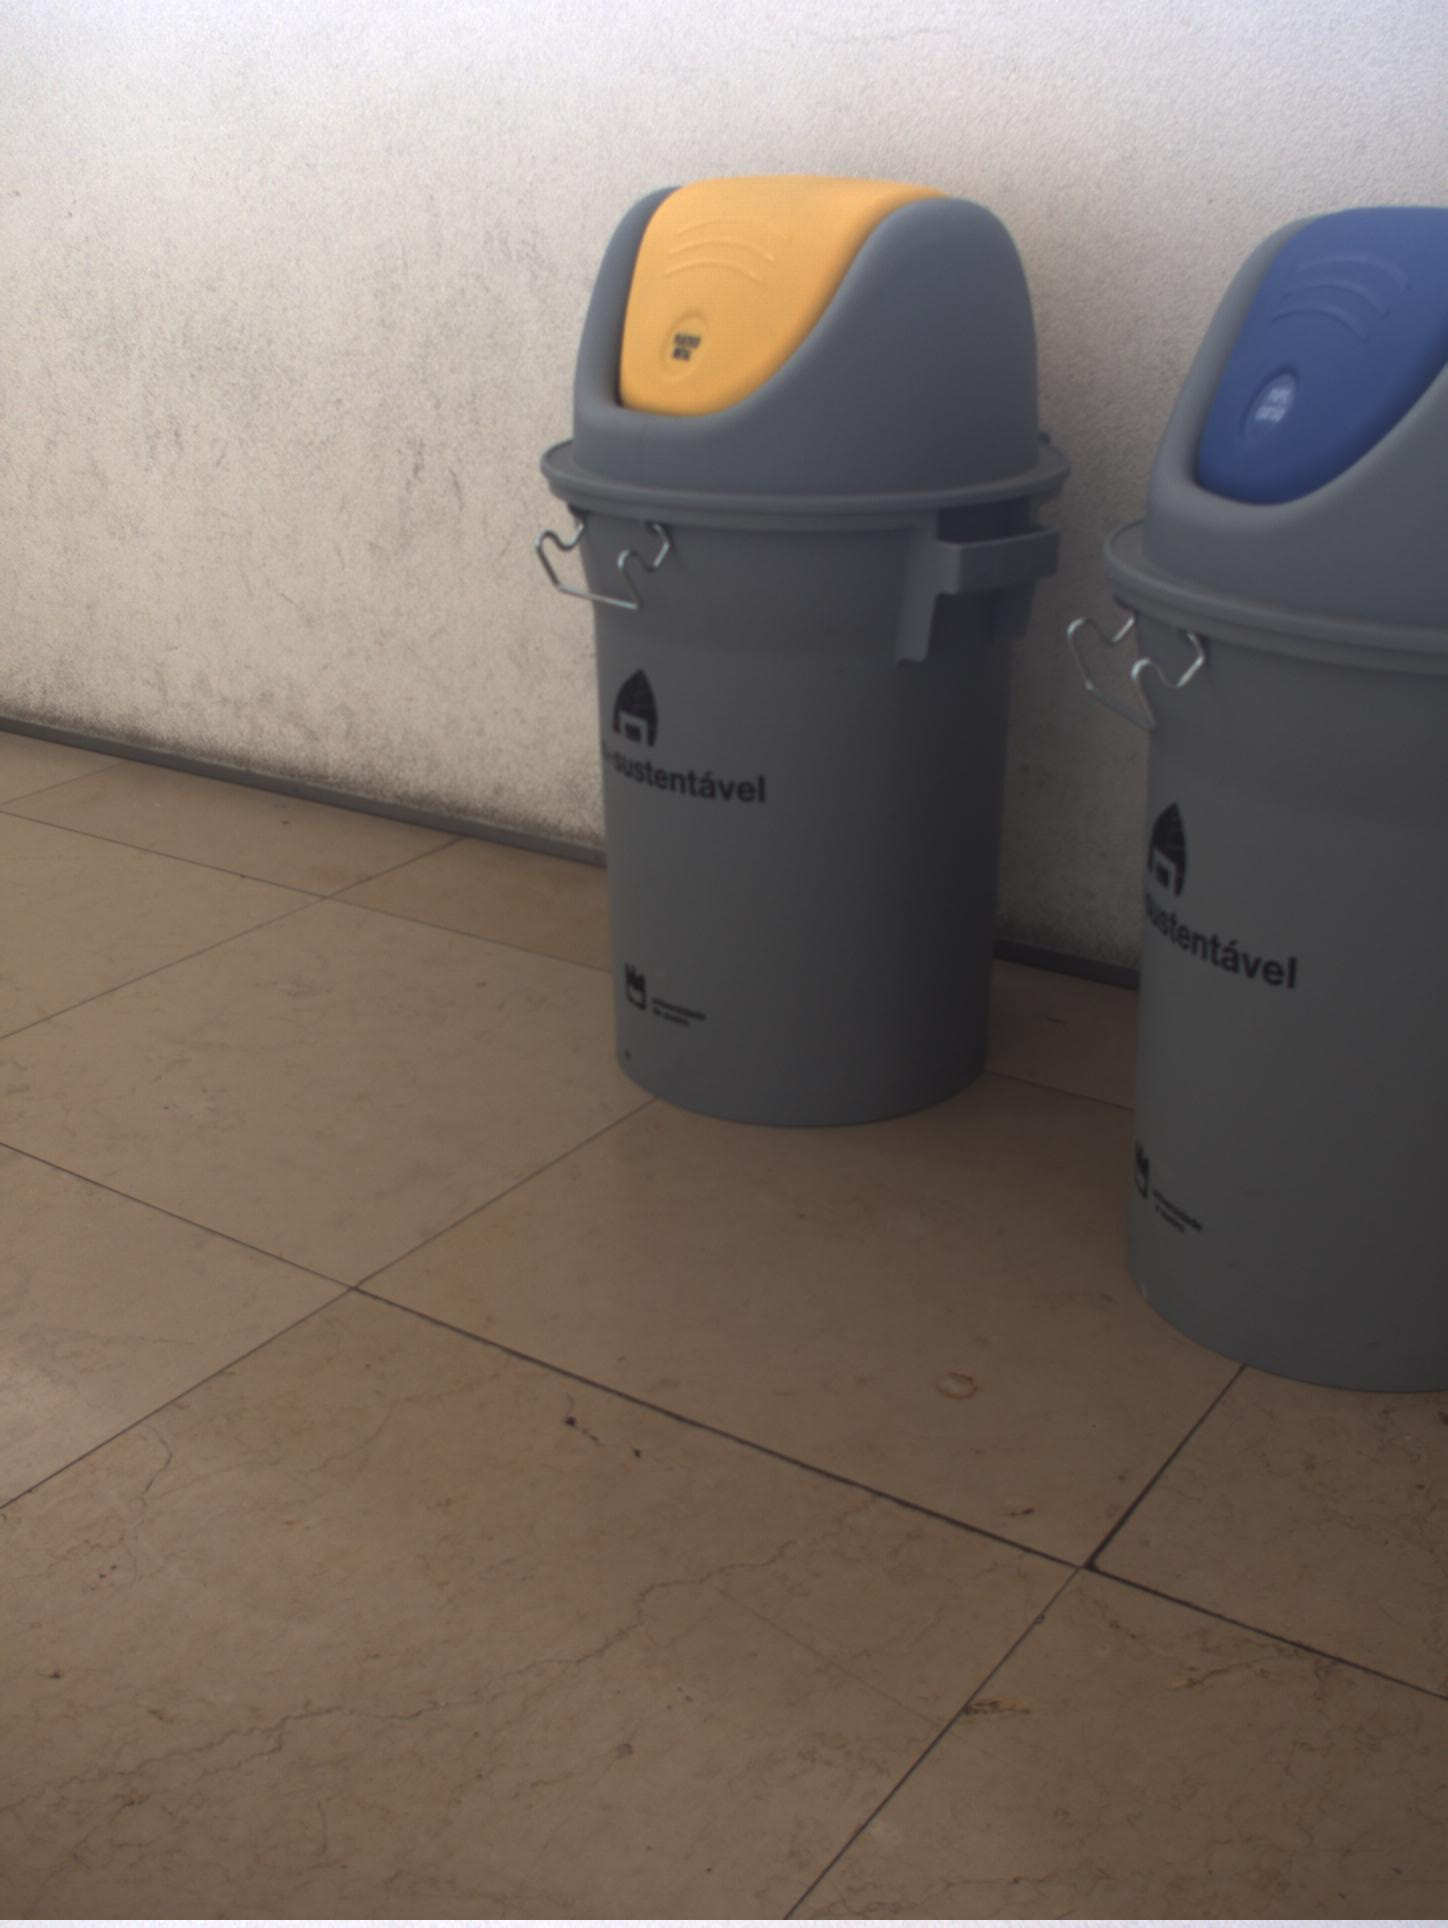
\includegraphics[width=0.6\textwidth]{illumination-issues-0}
    \end{subfigure}%
    \begin{subfigure}{0.5\textwidth}
        \centering
        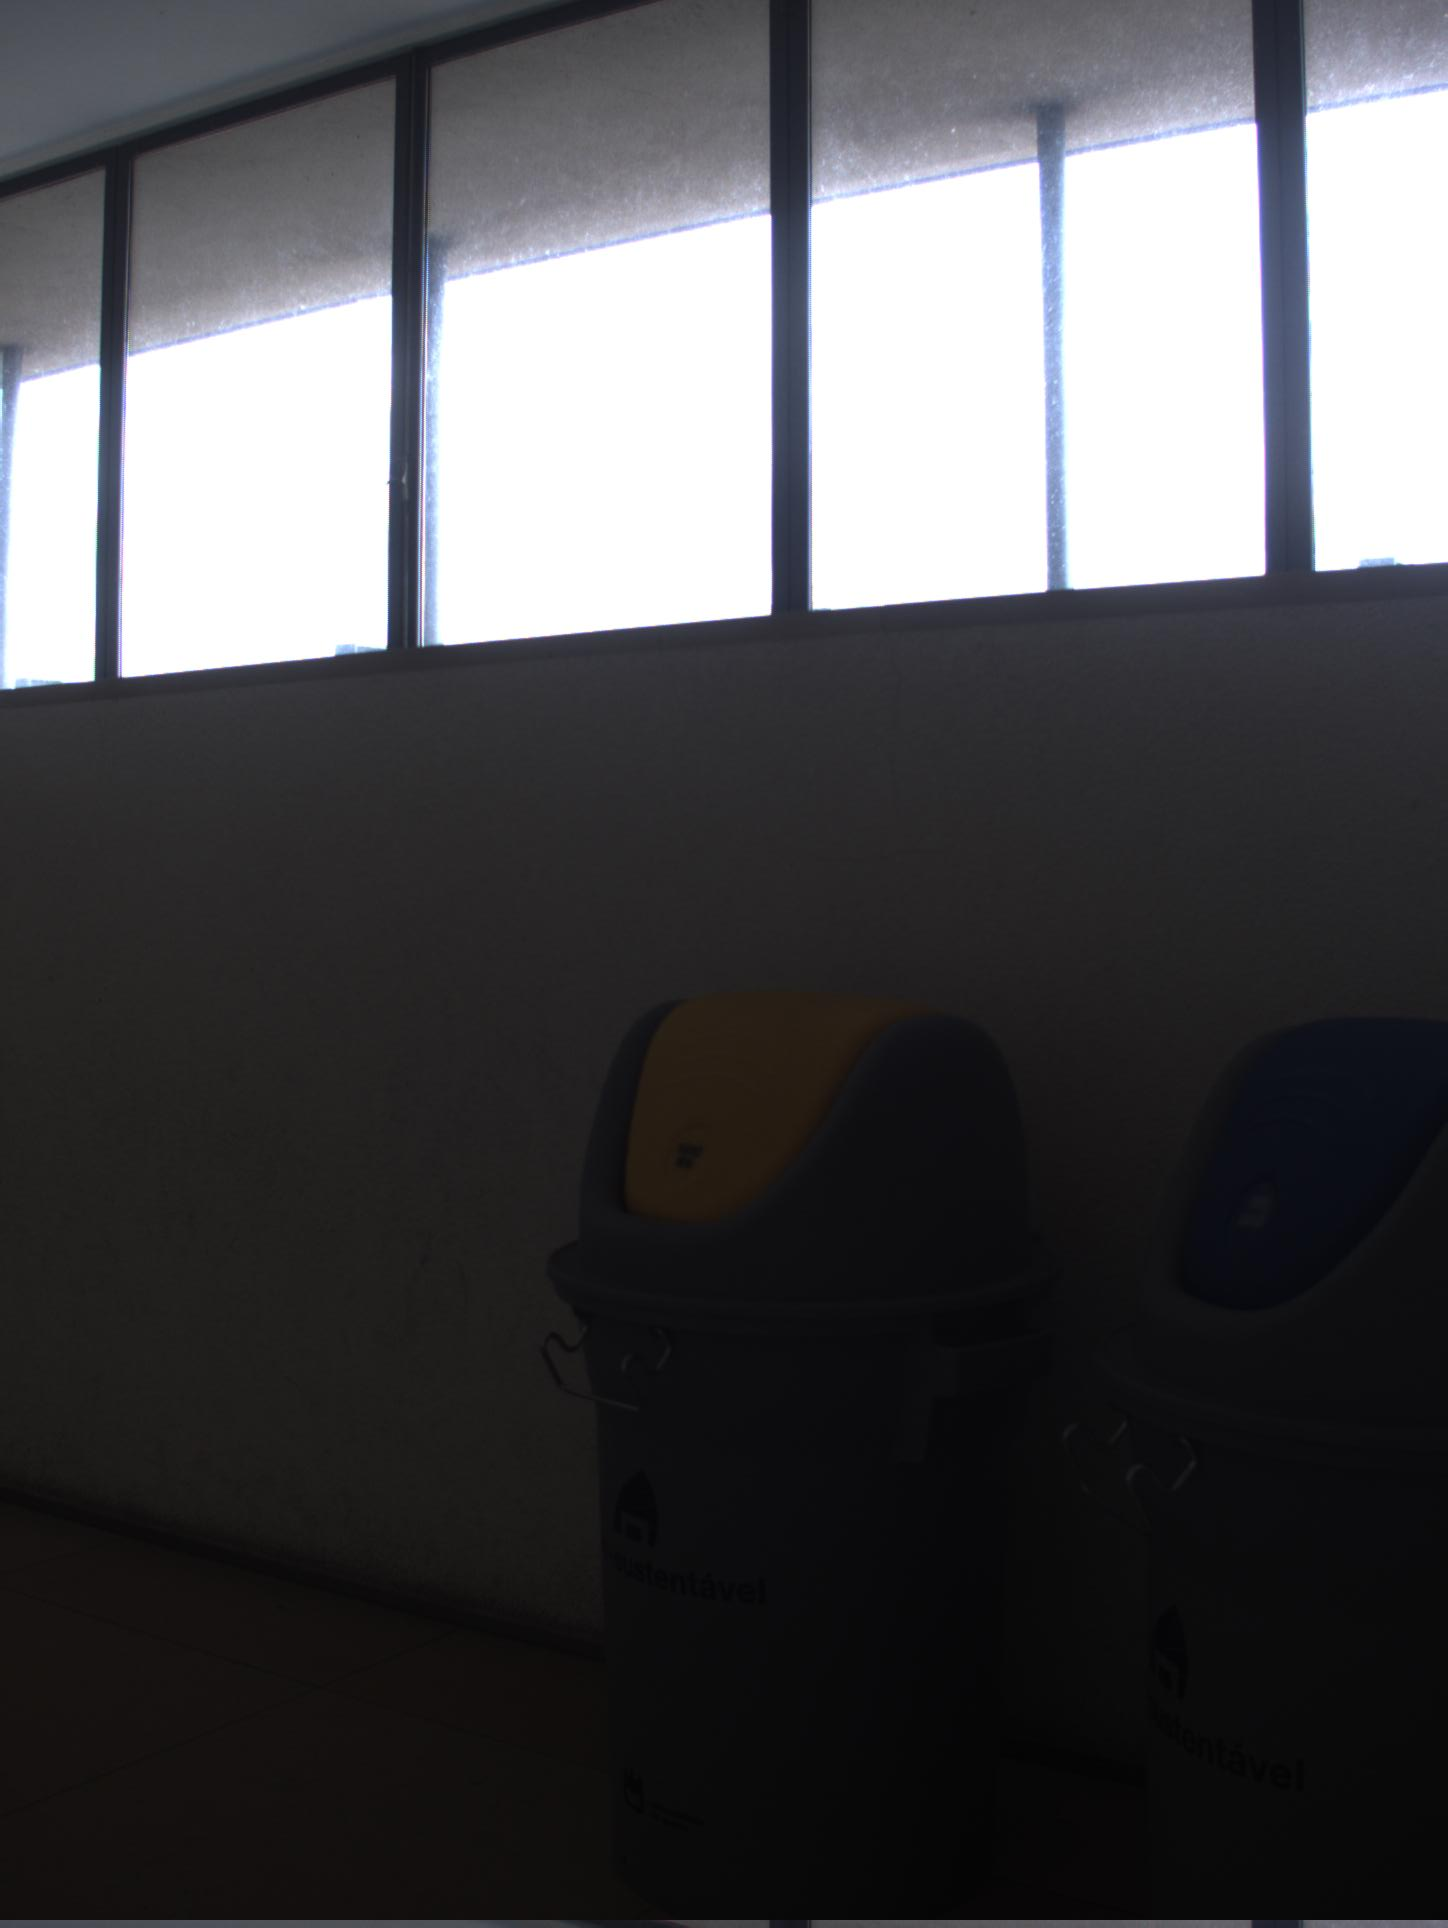
\includegraphics[width=0.6\textwidth]{illumination-issues-1}
    \end{subfigure}%

    \caption{Two images taken on the same acquisition with different colors.}
    \label{figure:illumination-issues-images}

\end{figure}

\begin{figure}[h]
    
    \centering
    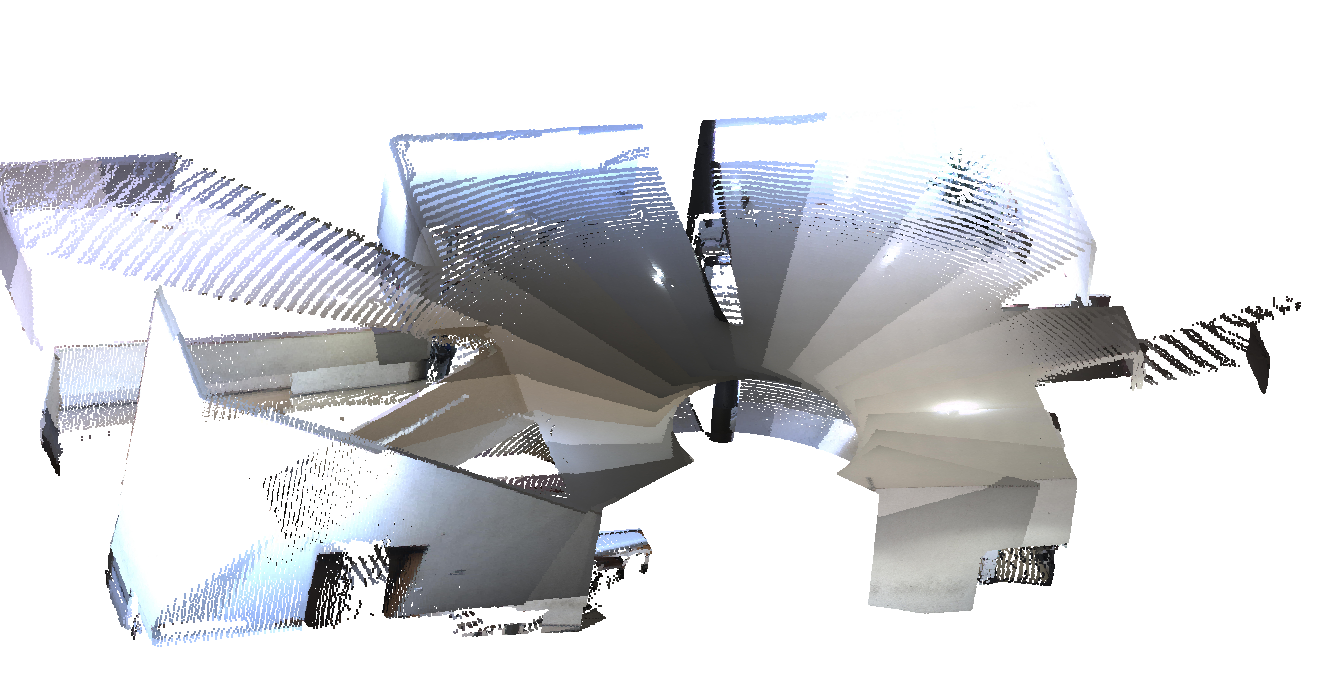
\includegraphics[width=0.8\textwidth]{color-registration-mean-4}

    \caption{Illumination issues in the point cloud.}
    \label{figure:illumination-issues-pointcloud}

\end{figure}

The color fusion techniques also have a great effect on the final result. The colors look sharper if the chosen method is the first or last color fusion method, but discontinuities caused by the imperfect registration are more noticeable. On the other hand, mean methods results in a blurring effect on the colors, but the discontinuities are less noticeable. In general, the mean fusion produces the best result overall, but the small details are smudged. The closest color fusion produces the sharpest result, so the small details are visible, however, it yields the worst quality overall. The two results can be seen in \cref{figure:fusion-methods-closest,figure:fusion-methods-mean}.

\begin{figure}[h]
    
    \centering
    \begin{subfigure}[t]{0.7\textwidth}
        \centering
        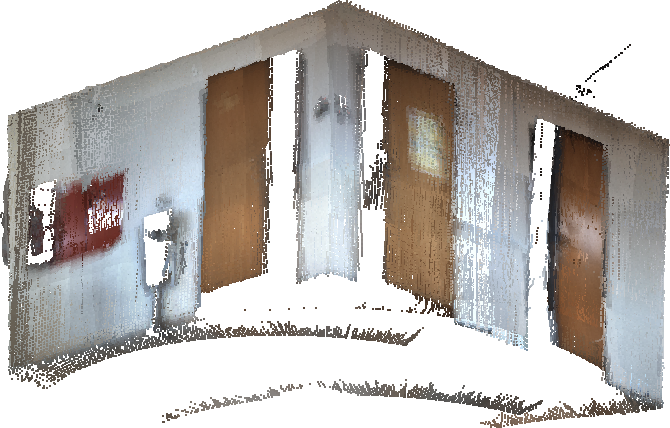
\includegraphics[width=0.9\textwidth]{color-registration-2}

        \caption{Mean color fusion method.}
        \label{figure:fusion-methods-mean}
    \end{subfigure}

    \begin{subfigure}[t]{0.7\textwidth}
        \centering
        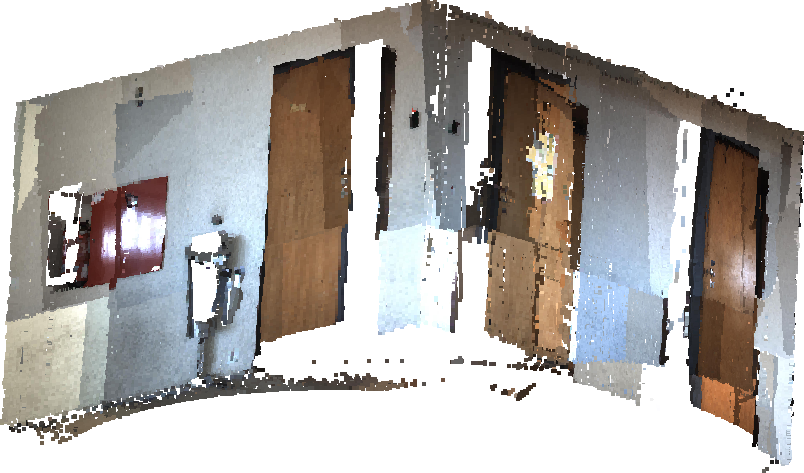
\includegraphics[width=0.9\textwidth]{color-registration-5}

        \caption{Closest color fusion method.}
        \label{figure:fusion-methods-closest}
    \end{subfigure}%

    \caption{Comparison of two color fusion methods.}
    \label{figure:fusion-methods-1}

\end{figure}

Moreover, the mean method still shows some discontinuities and edges. To improve the blending of the colors, this work proposes a weighted mean, based on two factors: $f_1$ and $f_2$. This factors prioritize colors that are taken closer to the point or taken closer to the center point of the camera. In \cref{figure:fusion-methods-f1,figure:fusion-methods-f2}, this two color fusion methods are compared against the closest color method, present in \cref{figure:fusion-methods-mean}. As seen, both methods have overall better results, specially in the blending of the different colors, and reducing the transitions between images.

\begin{figure}[h]
    
    \centering
    \begin{subfigure}[t]{\textwidth}
        \centering
        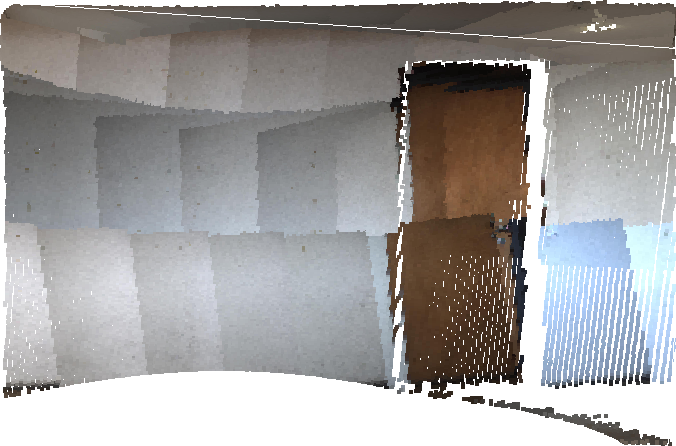
\includegraphics[width=0.6\textwidth]{color-registration-comparizon-last}

        \caption{Last color fusion method.}
        \label{figure:fusion-methods-mean}
    \end{subfigure}

    \begin{subfigure}[t]{\textwidth}
        \centering
        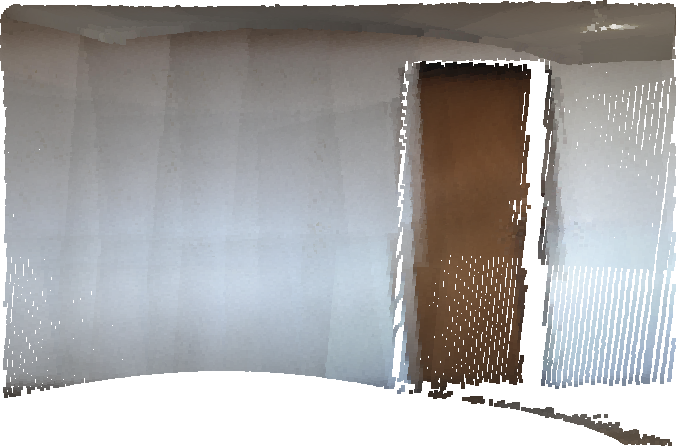
\includegraphics[width=0.6\textwidth]{color-registration-comparizon-f1}

        \caption{Weighted mean with factor $f_1$ color fusion method.}
        \label{figure:fusion-methods-f1}
    \end{subfigure}%

    \begin{subfigure}[t]{\textwidth}
        \centering
        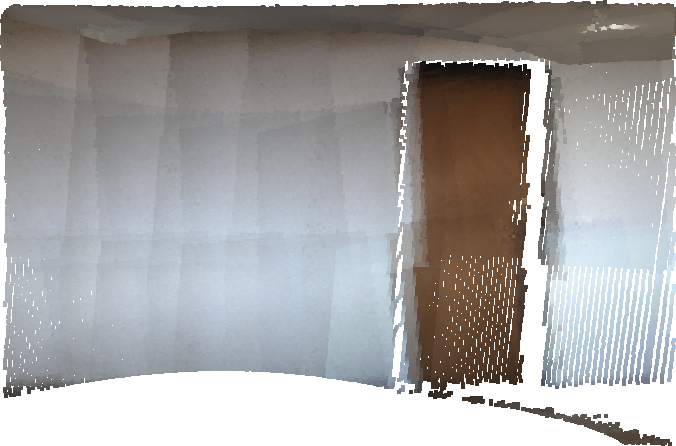
\includegraphics[width=0.6\textwidth]{color-registration-comparizon-f2}

        \caption{Weighted mean with factor $f_2$ color fusion method.}
        \label{figure:fusion-methods-f2}
    \end{subfigure}

    \caption{Comparison of two weighted mean color fusion methods.}
    \label{figure:fusion-methods-2}

\end{figure}

Finally, the color reconstruction method successfully colorized the point clouds, as seen in \cref{figure:full-color-registration}. However, the results are far from perfect, due to the inconsistent color in different images and the sub-optimal calibration of the camera.

\begin{figure}[h]
    
    \centering
    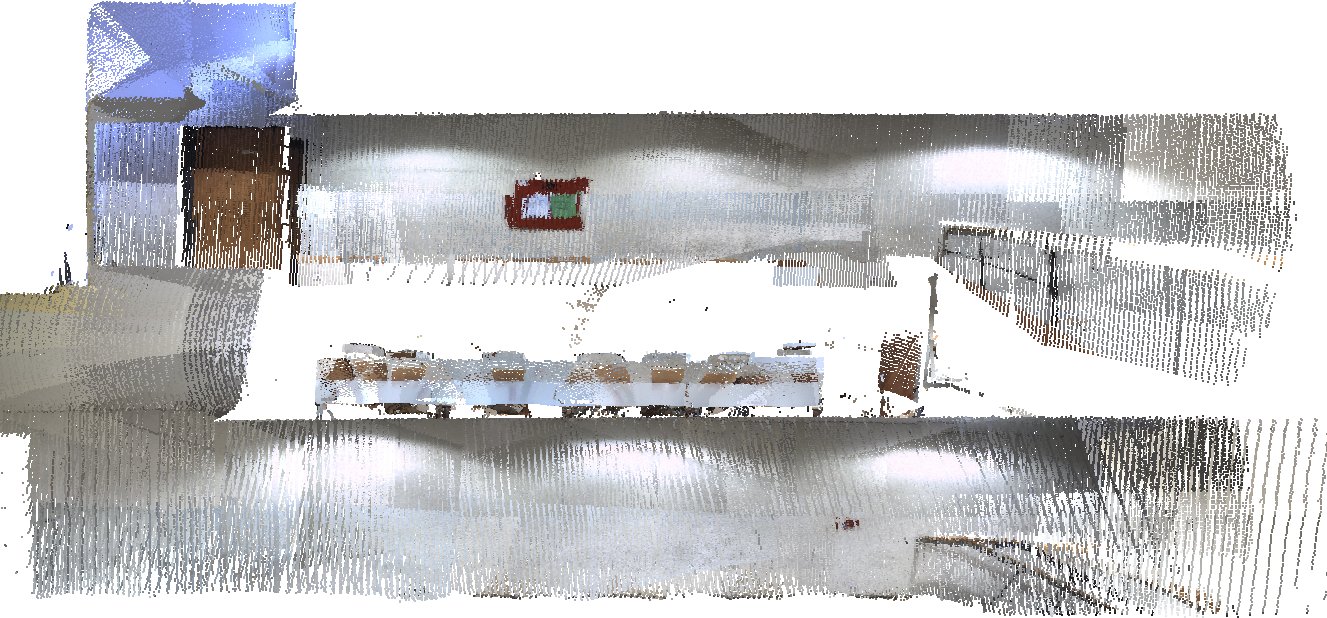
\includegraphics[width=\textwidth]{color-registration-last-3}

    \caption{Full color registration of one point cloud.}
    \label{figure:full-color-registration}
\end{figure}